% !TeX spellcheck = es_ES
%%%%  Las secciones de texto con fórmulas se separan con %%%%
%% Las fórmulas presentes entre 2 secciones de texto se separan con %%

%%%%%%%%%%%%%%%
%%  Capítulo 1: Introducción  %%
%%%%%%%%%%%%%%%
%%%%
\section{Reseña histórica}
\label{sec_intro_resenia}
%%%%

%%%%
Las bases de la teoría electromagnética clásica para el dominio macroscópico fueron formuladas por James Clerk Maxwell en 1873, en base al conocimiento previo desarrollado por Gauss, Ampère y Faraday, entre otros. Entre 1885 y 1887, Oliver Heaviside simplificó las expresiones e introdujo la notación vectorial actual, facilitando así la descripción matemática de los fenómenos físicos asociados \cite{Pozar:MwEngineering}.

En base a estos trabajos, Heinrich Hertz diseñó, entre 1886 y 1891, una serie de experimentos que validaron la teoría de ondas electromagnéticas propuesta por Maxwell. En 1886, Hertz construyó la primer antena dipolo, y en 1888, la primer antena parabólica, alimentada por un dipolo de 450 MHz, dando el puntapié inicial para el desarrollo de la radio durante la primera mitad del siglo \textsc{XX} \cite{Collin:GuidedWaves}.

El primer análisis de la propagación de ondas electromagnéticas en guías de ondas metálicas, publicado por Lord Rayleigh en 1897, y el posterior estudio teórico del comportamiento de ondas en guías dieléctricas por Debye y Hondros, en 1910, sentaron los cimientos para que, durante la década de 1930, comenzaran trabajos experimentales en transporte de ondas electromagnéticas en los laboratorios Bell \cite{Collin:GuidedWaves}.

Los conjuntos de antenas se popularizaron a partir de la aparición de la antena de Yagi-Uda en 1926, formada por elementos lineales que dan lugar a una fase fija. Durante la Segunda Guerra Mundial surgieron los conjuntos de antena de fase variable \cite{Stutzman:AntennaTheory}, y las guías de ondas y las antenas tomaron un lugar prioritario entre los ingenieros, matemáticos y físicos de la época, lo que incitó al desarrollo de métodos de análisis para facilitar la formulación de problemas con condiciones de borde complejas.

Recién finalizada la Segunda Guerra Mundial se comenzaron a fabricar circuitos \textit{microstrip}. En 1953, G. A. Deschamps presentó el primer trabajo sobre antenas con dicha tecnología, y la primer patente en ese sentido se registró en 1955 \cite{Balanis:Handbook}. Aún así, no fue hasta la década de 1970 que comenzaron a utilizarse en aplicaciones prácticas, principalmente gracias a la aparición de sustratos con bajas tangentes de pérdida, la mejora en técnicas de fotolitografía, y la optimización de modelos teóricos \cite{Barthia:Handbook}, que permitieron solucionar los problemas de dispersión y aparición de modos indeseados. Sin embargo, la simplificación constructiva trajo aparejados problemas de acoplamiento mutuo, que debieron ser abordados por técnicas de filtrado y blindaje.

\section{Ecuaciones de Maxwell}
\label{subsec_ecuaciones_maxwell}
%%%%
La teoría electromagnética propuesta por Maxwell, y simplificada por Heaviside, se reduce a cuatro ecuaciones diferenciales lineales vectoriales e interdependientes que, en notación diferencial, quedan expresadas como se observa a la izquierda de la ecuación \ref{eq:Maxwell} \cite{Pozar:MwEngineering}, donde $\vec{E}$ es el campo eléctrico, en $(V/m)$; $\vec{H}$ es el campo magnético, en $(A/m)$; $\vec{D}$ es la densidad de flujo eléctrico, en $(C/m^2)$; $\vec{B}$ es la densidad de flujo magnético, en $(Wb/m)$; $\vec{M}$ es la densidad de corriente magnética, en $(V/m)$, y se considera por completitud y simetría; $\vec{J}$ es la densidad de corriente eléctrica, en $(A/m^2)$; y $\rho$ es la densidad de carga eléctrica, en $(C/m^2)$.

\begin{align}
\label{eq:Maxwell}
\left.\begin{array}{rr@{\mskip\thickmuskip}l}
\text{Faraday} &\nabla \times \vec{E} & = -\frac{\partial \vec{B}}{\partial t} - \vec{M}\\
\text{Ampère} &\nabla \times \vec{H} & = \frac{\partial \vec{D}}{\partial t} + \vec{J} \\
\text{Gauss} &\nabla \cdot \vec{D} & = \rho \\
& \nabla \cdot \vec{B} & = 0
\end{array} \right\}
\quad \implies \quad
\left\{\begin{array}{r@{\mskip\thickmuskip}l}
\nabla \times \vec{E} & = -j \omega \vec{B} - \vec{M} \\
\nabla \times \vec{H} & = j \omega \vec{D} + \vec{J} \\
\nabla \cdot \vec{D} & = \rho\\
\nabla \cdot \vec{B} & = 0
\end{array}\right.
\end{align}

De las ecuaciones \ref{eq:Maxwell} se deduce que las fuentes de campo electromagnético son la densidad de carga eléctrica $\rho$ y las corrientes $\vec{M}$ y $\vec{J}$. Utilizando propiedades del cálculo vectorial es posible, además, deducir\footnote{Para ello se debe aplicar la divergencia a la ecuación de Ampère, y recordar que $\nabla \cdot (\nabla \times \vec{F}) = 0$.} la ecuación de continuidad \ref{eq:continuidad}.

\begin{align}
	\label{eq:continuidad}
	\nabla \cdot \vec{J} + \frac{\partial \rho}{\partial t} &= 0.
\end{align}


A partir de las ecuaciones de Maxwell (\ref{eq:Maxwell}), y considerando relaciones constitutivas que no varían en el tiempo ni en función de la frecuencia (es decir, no hay dispersión), y donde no hay cargas libres ni corrientes ($\rho=0$ y $\vec{J}=0$), donde el material es isótropo y macroscópico, y donde no se consideran pérdidas, es posible, utilizando la linealidad de dichas ecuaciones, separar el comportamiento en el tiempo y en el espacio, expandiendo los campos en modos armónicos y expresándolos como combinaciones lineales de los mismos. Los modos, entonces, resultan de un patrón espacial ($\vec{H}(\vec{r})$ o $\vec{E}(\vec{r})$) multiplicado por un patrón temporal.

Dado que la mayor parte del análisis se realiza sobre campos de comportamiento armónico y en régimen permanente, la dependencia del tiempo de la ecuaciones de Maxwell se suele simplificar, de manera que la dependencia temporal, $e^{j \omega t}$, suele quedar implícita, dado que resulta común para todos los términos. Así, las derivadas respecto del tiempo resultan más sencillas, y los vectores de campos se vuelven funciones vectoriales complejas dependientes sólo de coordenadas espaciales \cite{Collin:GuidedWaves}. El resultado de esta simplificación se observa en el lado derecho de la ecuación \ref{eq:Maxwell}.

Bajo estas consideraciones, resulta claro que las configuraciones posibles de campo son transversales: Para cualquier campo magnético $\vec{H}(\vec{r}) = \vec{a} \exp(j \vec{\beta} \cdot \vec{r})$, la ecuación de la divergencia del mismo obliga a que $\vec{a} \cdot \vec{\beta} = 0$.

\subsection{Campos en medios materiales}
\label{subsec_campos_en_dielectricos}

Un campo eléctrico aplicado sobre cualquier material dieléctrico genera una polarización de sus átomos y/o moléculas, creando momentos dipolares eléctricos (o alineándolos, si en el material existían previamente), y dando lugar a un vector de polarización adicional, $\vec{P}_e$, que genera un decrecimiento en el campo eléctrico total presente en el material. En el mismo sentido, un campo magnético aplicado sobre un medio material podría ser capaz de alinear los momentos dipolares magnéticos en un material magnético, produciendo un vector de polarización magnética $P_m$. Si el medio es, además, lineal e isotrópico, dichas polarizaciones son proporcionales al campo aplicado, de forma que $\vec{P}_e = \epsilon_0 \chi_e \vec{E}$ y $\vec{P}_m = \chi_m \vec{H}$, con $\chi_e$ y $\chi_m$ las susceptibilidades eléctrica y magnética, respectivamente. Dado que las mismas toman valores complejos, los medios materiales poseen permitividades eléctricas y permeabilidades magnéticas también complejas, asociadas a las pérdidas debidas al amortiguamiento causado por los momentos dipolares respectivos \cite{Fernandez:Electromag}. Las relaciones constitutivas resultan, entonces,

\begin{subequations}
	\label{eq:polarization_vector}
	\begin{align}
		\vec{D} = \epsilon_0 \vec{E} + \vec{P}_e = \epsilon_0 (1+\chi_e)\vec{E} = \epsilon \vec{E} &= (\epsilon' - j \epsilon'') \vec{E} y\\
		\vec{B} = \mu_0 (\vec{H} + \vec{P}_m) = \mu_0 (1+\chi_m)\vec{H} = \mu \vec{H} &= (\mu' - j \mu'') \vec{H}.
	\end{align}
\end{subequations}

Si, además, el material posee una conductividad $\sigma$, la aplicación de un campo eléctrico da lugar a la aparición de una densidad de corriente $\vec{J}$, que en algunos casos, cuando $\sigma$ es independiente del campo eléctrico aplicado, se puede expresar, según la ley de Ohm, como

\begin{align}
	\label{eq:ohms_law}
	\vec{J} &= \sigma \vec{E}.
\end{align}

La ecuación de Ampère de \ref{eq:Maxwell} queda, entonces, expresada como
\begin{subequations}
	\begin{align}
		\nabla \times \vec{H} & = j \omega \vec{D} + \vec{J} = j \omega \epsilon \vec{E} + \sigma \vec{E} = j \omega \epsilon' \vec{E} + (\omega \epsilon'' + \sigma)\vec{E}\\
		& = j \omega \left( \epsilon' - j\epsilon'' - j \frac{\sigma}{\omega} \right) \vec{E}.
	\end{align}
\end{subequations}

La relación entre la parte imaginaria y la parte real de la corriente total de desplazamiento se conoce como tangente de pérdidas \cite{Pozar:MwEngineering}:

\begin{align}
	\label{eq:tan_perdidas}
	\tan \; \delta &= \frac{\omega \epsilon'' + \sigma}{\omega \epsilon'}.
\end{align}

Cuando el material no es homogéneo, los coeficientes $\epsilon$ y $\mu$ dependen de la posición. Si, además, el material es anisotrópico, como en el caso de los cristales y gases ionizados, la relaciones expresadas antes entre los vectores de polarización ($\vec{P}_e$ y $\vec{P}_m$) y los campos no se cumplen, sino que deben ser expresadas como tensores de rango 2 (diadas), como se muestra en la ecuación \ref{eq:diadas}, explicitando así su dependencia de la dirección \cite{Collin:GuidedWaves}. Si, además, el material no es lineal, los coeficientes $\epsilon_{ij}$ y $\mu_{ij}$ pueden ser funciones de $\vec{E}$ y $\vec{H}$ respectivamente.

\begin{equation} \label{eq:diadas}
\begin{bmatrix}
D_x \\
D_y \\
D_z
\end{bmatrix}
=
\begin{bmatrix}
\epsilon_{xx} & \epsilon_{xy} & \epsilon_{xz} \\
\epsilon_{yx} & \epsilon_{yy} & \epsilon_{yz} \\
\epsilon_{zx} & \epsilon_{zy} & \epsilon_{zz}
\end{bmatrix}
\begin{bmatrix}
E_x \\
E_y \\
E_z
\end{bmatrix}
\qquad\text{y}\qquad
\begin{bmatrix}
B_x \\
B_y \\
B_z
\end{bmatrix}
=
\begin{bmatrix}
\mu_{xx} & \mu_{xy} & \mu_{xz} \\
\mu_{yx} & \mu_{yy} & \mu_{yz} \\
\mu_{zx} & \mu_{zy} & \mu_{zz}
\end{bmatrix}
\begin{bmatrix}
H_x \\
H_y \\
H_z
\end{bmatrix}
\end{equation}

\subsection{Análisis de automodos}
\label{sec:automodos}

Las ecuaciones del rotor de las ecuaciones de Maxwell (\ref{eq:Maxwell}) pueden ser desacopladas\footnote{El desacople se realiza de la siguiente manera:
	\begin{align*}
		\nabla \times \vec{H}(\vec{r}) + j\omega\vec{D}(\vec{r}) = 0 \\
		\frac{1}{\epsilon_r} \nabla \times \vec{H}(\vec{r}) + j\omega\epsilon_0\vec{E}(\vec{r}) = 0 \\
		\nabla \times \left(\frac{1}{\epsilon_r} \nabla \times \vec{H}(\vec{r})\right)= - \nabla \times (j\omega\epsilon_0\vec{E}(\vec{r})) = -j \omega\epsilon_0 \nabla \times \vec{E}(\vec{r}) \\
		\nabla \times \left(\frac{1}{\epsilon_r} \nabla \times \vec{H}(\vec{r})\right) = -j \omega\epsilon_0 \mu \vec{H}(\vec{r})
	\end{align*}
	
	}, de manera que resulte la ecuación
	
	\begin{align}
		\label{eq:master-eq}
		\nabla \times \left(\frac{1}{\epsilon_r} \nabla \times \vec{H}(\vec{r}) \right) = \left(\frac{\omega}{c}\right)^2 \vec{H}(\vec{r}).
	\end{align}

Una expresión similar se puede obtener para el campo eléctrico. Sin embargo, también es posible obtener el campo eléctrico a partir de la ecuación de divergencia, una vez resuelta la ecuación \ref{eq:master-eq},

\begin{align}
	\vec{E}(\vec{r}) = \frac{j}{\omega \epsilon_0 \epsilon_r} \nabla \times \vec{H}(\vec{r}).
\end{align}

La ecuación \ref{eq:master-eq} es una ecuación de autovalores: El lado izquierdo puede ser considerado un operador, $\hat{\Theta}$, de manera que

\begin{align}
	\hat{\Theta} \vec{H}(\vec{r}) = \left(  \frac{\omega}{c} \right)^2 \vec{H}(\vec{r}),
\end{align}

donde los autovectores son los valores que toma $\vec{H}(\vec{r})$, es decir, los patrones espaciales, y los autovalores son $(\omega/c)^2$, relacionados a las frecuencias de esos modos. El operador $\hat{\Theta}$ es lineal\footnote{Es posible demostrar que, además, el operador es hermítico, lo que permite deducir que: los autovalores serán siempre no-negativos, y por lo tanto las frecuencias $\omega$ serán siempre reales; cualesquiera dos modos armónicos de diferentes frecuencias serán siempre ortogonales, y los modos que comparten frecuencia, los modos degenerados, surgen por las simetrías e invariancias del medio; y que se cumple el teorema variacional, que indica que los autovalores más pequeños coinciden con los modos de menor energía \cite{Joannopoulos:PhotonicCrystals}.}, de manera que cualquier combinación lineal de soluciones es también solución. Este acercamiento a las ecuaciones de Maxwell permite resolver problemas tridimensionales, especialmente los relacionados a estructuras resonantes cerradas y estructuras periódicas.

\subsection{Condiciones de borde} \label{sec:condiciones-borde}

\begin{figure}[htp]
	\centering
	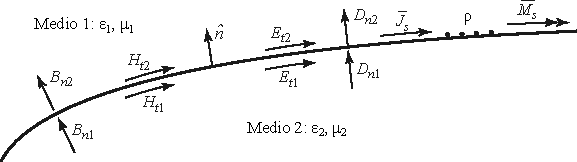
\includegraphics[width=0.8\textwidth]{intro_electro/condiciones_borde.pdf}
	\caption{Corrientes, campos y carga superficial en una interfaz general entre dos medios \cite{Pozar:MwEngineering}.}.
	\label{fig:condiciones_borde}
\end{figure}

Si se considera una interfaz entre dos medios, como la que se muestra en la figura \ref{fig:condiciones_borde}, a partir de las ecuaciones de Maxwell y los teoremas integrales, se pueden deducir las siguientes condiciones de borde:
\begin{subequations}
	\label{eq:condiciones_borde}
	\begin{align}
		\hat{n} \cdot (\vec{D}_{2} - \vec{D}_{1}) & = \rho_s \\
		\hat{n} \cdot (\vec{B}_{2} - \vec{B}_{2}) & = 0 \\
		\hat{n} \times (\vec{E}_2 - \vec{E}_1)  & = - \vec{M}_s \\
		\hat{n} \times (\vec{H}_2 - \vec{H}_1) & = \vec{J}_s
	\end{align}
\end{subequations}

%\paragraph{Campos sobre una superficie dieléctrica}
%Dado que en una interfaz entre dos dieléctricos no hay carga eléctrica ni densidades de corriente, las ecuaciones \ref{eq:condiciones_borde} establecen que las componentes normales de los vectores $\vec{D}$ y $\vec{B}$ se conservan, y que las componentes tangenciales de $\vec{E}$ y $\vec{H}$ también lo hacen.

%\paragraph{Campos sobre una superficie conductora eléctrica}
%Si el conductor no tiene pérdidas ($\sigma \rightarrow \infty$), todos los campos deben ser cero en su interior \footnote{La profundidad de penetración, definida en secciones siguientes, se anula.}. Considerando, además, que $\vec{M}_s = 0$, la componente tangencial del campo eléctrico, $E_t$ desaparece sobre la superficie del conductor. Dado que la diferencia entre las componentes normales del campo magnético está dada por $\vec{J}_s$, y el campo magnético debe anularse en el conductor, la densidad de corriente superficial está dada únicamente por el campo magnético externo al mismo. En el mismo sentido, la densidad de carga superficial $\rho_s$ es la expresión, sobre la superficie del conductor, de la componente normal de $\vec{D}$.

% SKIN DEPTH

%\paragraph{Campos sobre una superficie conductora magnética}
%Dado que la superficie conductora magnética representa el caso dual al de la superficie conductora eléctrica, en este caso se espera que la componente tangencial de $\vec{H}$ se anule sobre la superficie, mientras que la componente tangencial del campo eléctrico dé lugar a corrientes magnéticas sobre la misma.

%%%%% QUEDA DECRI QUE PASA CON UNA CORRIWENTE EN HORIZRAON O VERTICAL - LIBRO DE YAMAT, PAG 10.
%% COMPLETAR CON COLLIN %%

\section{Ecuación de onda}
\label{subsec_eq_de_onda}
%%%%

Al considerar una región del espacio lineal, isotrópica y homogénea, se puede calcular el rotor de la primera ecuación de Maxwell y aplicar la segunda\footnote{Se deberá utilizar la identidad $\nabla \times \nabla \times \vec{E} = \nabla \nabla \cdot \vec{E} - \nabla^2\vec{E}$, donde $\nabla \cdot \vec{E} = \rho/\epsilon$. Aplicando, además, lo mismo para el campo magnético, y considerando que $\nabla \cdot \vec{B} = 0$: \newline % OJO QUE PUEDE ROMPER TODO
	
	
	\begin{tabular}{ r l | r l }
		 $\nabla \times \nabla \times \vec{E}$ & $=\; -j \omega \mu \nabla \times \vec{H} - \nabla \times \vec{M}$ & $\nabla \times \nabla \times \vec{H}$ & $=\; j \omega \nabla \times \vec{D} +  \nabla \times \vec{J}$ \\
		 $\nabla \nabla \cdot \vec{E} - \nabla^2 \vec{E}$ & $=\; -j \omega \mu \nabla \times \vec{H} - \nabla \times \vec{M}$ & $\nabla \nabla \cdot \vec{H} - \nabla^2 \vec{H}$ & $=\; j \omega \epsilon \nabla \times \vec{E} + \nabla \times \vec{J}$ \\
		 $\frac{\nabla \rho}{\epsilon} - \nabla^2 \vec{E}$ & $=\; \omega^2 \mu \epsilon \vec{E} - j \omega \mu \vec{J} - \nabla \times \vec{M}$ & $\frac{1}{\mu} \nabla (\cancelto{0}{\nabla \cdot \vec{B}}) - \nabla^2 \vec{H}$ & $=\; j \omega \epsilon (-j \omega \vec{B} - \vec{M}) + \nabla \times \vec{J}$ \\
		 $\nabla^2 \vec{E} + \omega^2 \mu \epsilon \vec{E}$ & $=\; j \omega \mu \vec{J} + \frac{\nabla \rho}{\epsilon} + \nabla \times \vec{M}$ & $\nabla^2 \vec{H} + \omega^2 \epsilon \mu \vec{H}$ & $=\;  j \omega \epsilon \vec{M} - \nabla \times \vec{J}$
	\end{tabular}	
	}, lo que da como resultado las expresiones \footnote{De estas ecuaciones, se observa que el campo magnético está determinado por la componente rotacional de la corriente eléctrica, mientras que el campo eléctrico está determinado por todas las componentes de la misma. De manera análoga, se cumple la relación inversa para el caso de la corriente magnética.}:

\begin{subequations}
	\begin{align}
		\nabla^2 \vec{E} + \omega^2 \epsilon \mu  \vec{E} & = j \omega \mu \vec{J} + \frac{\nabla \rho}{\epsilon} + \nabla \times \vec{M} \label{eq:eq_ondas_completa_E} \\
		\nabla^2 \vec{H} + \omega^2 \epsilon \mu \vec{H} & =  j \omega \epsilon \vec{M} - \nabla \times \vec{J}. \label{eq:eq_ondas_completa_H}
	\end{align}
	\label{eq:eq_ondas_completa_E_H}
\end{subequations}

Si, además, la región del espacio es libre de fuentes ($J=0$, $M=0$ y $\rho=0$), se deducen las ecuaciones de Helmholtz para ambos campos, donde $\gamma$ es el número de onda, en unidades de $(1/m)$:

\begin{equation}
	\label{eq:Helmholtz}
	\begin{aligned}
		\nabla^2  \vec{E} + \gamma^2 \vec{E} &= 0  \\
		\nabla^2 \vec{H} + \gamma^2 \vec{H}& = 0. 
	\end{aligned}
\end{equation}
%%%%

Para el caso sin pérdidas se puede expresar como $\gamma = \beta = \omega \sqrt{\mu \epsilon}$, mientras que si se considera que existen pérdidas óhmicas,  su efecto puede ser tenido en cuenta si  $\gamma$ asume un valor complejo, tal que

\begin{align}
\label{eq:constante-propagacion-compleja}
\gamma = -j\alpha + \beta &= j\omega \sqrt{\mu (\epsilon'-j\epsilon'') - j \sigma \epsilon/\omega}.
\end{align}

Para el caso de un buen conductor, la expresión de $\gamma$ resulta

\begin{align}
\gamma = -j\alpha + \beta &= j \omega \sqrt{\mu \epsilon} \sqrt{\sigma/(\omega \epsilon)} = (1+j) \sqrt{\omega \mu \sigma/2},
\end{align}

lo que nos permite definir la profundidad de penetración como 

\begin{align}
\label{eq:prof_penetacion}
\delta_s = -1/\alpha &= \sqrt{\frac{2}{\omega \mu \sigma}}.
\end{align}

En coordenadas cartesianas, para resolver las ecuaciones \ref{eq:Helmholtz} resulta sencillo aplicar el método de separación de variables\footnote{En coordenadas cartesianas, $\nabla^2 E = \frac{\partial^2 \vec{E}}{\partial x^2} + \frac{\partial^2 \vec{E}}{\partial y^2} + \frac{\partial^2 \vec{E}}{\partial z^2}$. Reemplazando las coordenadas $E_i$ de $\vec{E}, para i=x,y,z$ por funciones $f(x),g(y),h(z)$ independientes entre sí, se obtiene que $\frac{f''(x)}{f(x)} + \frac{g''(y)}{g(y)} + \frac{h''(z)}{h(z)} + \beta_0^2 = 0$. Como las funciones $f$,$g$ y $h$ son independientes, se deduce que $\frac{f''(x)}{f(x)} = -\beta_x^2$, $\frac{g''(y)}{g(y)} = -\beta_y^2$ y $\frac{h''(z)}{h(z)} = -\beta_z^2$.}, que da lugar a ecuaciones cuya solución es de la forma $e^{\pm j \beta_i i}$, con $i = x, y$ o $z$, respectivamente. Las soluciones con un signo positivo en el exponente corresponden a ondas que viajan en la dirección negativa ($-x, -y, -z$), mientras que las que tienen un signo negativo corresponden a ondas que viajan en la dirección positiva. Dado que ambas soluciones son válidas y posibles, en función de las condiciones de borde, en general la expresión de la propagación de los campos electromagnéticos quedará establecida como la suma de ambas, afectadas por un factor de amplitud dependiente de la coordenada evaluada.

Para el caso de ondas que viajan en la dirección positiva,

\begin{equation}
	\label{eq:electric_field_wave_solution}
	\vec{E}(x,y,z) = \vec{E}_0 \;e^{-j(\gamma_x x + \gamma_y y + \gamma_z z)} = \vec{E}_0 \;e^{-j\vec{\gamma}\cdot\vec{r}},
\end{equation}

donde se consideró que $\vec{E}_0 = A \hat{x} + B \hat{y} + C \hat{z}$, $\vec{r} = x \hat{x} + y \hat{y} + z \hat{z}$ y

\begin{equation}
\label{eq:numero_de_onda}
\gamma_x^2 + \gamma_y^2 + \gamma_z^2 = \gamma^2. \\
\end{equation}


Al expresar la divergencia del campo eléctrico de la ecuación \ref{eq:electric_field_wave_solution}, se obtiene\footnote{Aplicando $\nabla \cdot (f \vec{A}) = \vec{A} \cdot \nabla f + f \nabla \cdot \vec{A}$ a la expresión, resulta $\nabla \cdot \vec{E} = \vec{E}_0 \cdot \nabla e^{-j \vec{\beta} \vec{r}} + e^{-j \vec{\beta} \vec{r}}\nabla \cdot \vec{E}_0$, donde $\nabla \cdot \vec{E}_0 =0$}


\begin{align}
\nabla \cdot \vec{E} = \nabla \cdot \vec{E}_0 e^{-j\vec{\gamma} \cdot \vec{r}} & = -j \vec{\gamma} \cdot \vec{E}_0 e^{-j \vec{\gamma} \cdot \vec{r}} = 0,
\end{align}

de lo que se puede deducir que $\vec{\gamma} \cdot \vec{E}_0 = 0$, de modo que el campo eléctrico, en una onda plana, es siempre perpendicular a la dirección de propagación.

De la ecuación de Faraday de \ref{eq:Maxwell}, considerando espacio libre de cargas, se obtiene que, para una onda plana en un medio sin pérdidas, el campo magnético es siempre ortogonal al campo eléctrico y a la dirección de propagación, y que los campos están relacionados de forma que \cite{Fernandez:Electromag}

\begin{align}
	\label{eq:relacion-e-h-ondaplana}
	\vec{H}(\vec{r},t) &= \pm \frac{\hat{\beta} \times \vec{E}(\vec{r},t)}{\eta},
\end{align}

donde $\eta$ es la impedancia de onda, que tiene la forma

\begin{align}
	\eta &= \frac{j \omega \mu}{\gamma }.
\end{align}

Para el caso con pérdidas, y considerando que la dirección de propagación es $z$, las componentes $x$ e $y$ se comportan como

\begin{equation}
E_i(z) = E_i \; e^{-j\gamma z} = E_i \; e^{-\alpha z} \; e^{-j \beta z}, \quad i=x,y. \nonumber
\end{equation}

Si el medio es el vacío, la impedancia intrínseca se denota $\eta_0$ y tiene un valor de $377\; \Omega$, mientras que para otros materiales está determinada por su permitividad eléctrica y permeabilidad magnética, y puede ser compleja si hay pérdidas.

La velocidad de fase se define como $v_p=\omega/\beta$, que de no haber pérdidas queda como $1/\sqrt{\mu \epsilon}$, y que para el caso particular del vacío, se expresa como $1/\sqrt{\mu_0 \epsilon_0} = c$, donde $c$ es la velocidad de la luz en el vacío. Así, la velocidad de fase en cualquier medio material sin pérdidas resulta $c/\sqrt{\epsilon_r \mu_r}$.

La velocidad de grupo, en tanto, se define como $v_g = d\omega/d\beta$, y representa la velocidad a la que una envolvente de onda se propaga en el espacio. Para el caso en que no existe dispersión, la velocidad de fase y la velocidad de grupo coinciden, pues la derivada que define a la velocidad de grupo es constante.

La longitud de onda, $\lambda$, es la distancia espacial entre dos máximos sucesivos, por lo que se expresa como $\lambda = 2\pi / \beta = v_p/f$.

\section{Guias de ondas}
\label{subsec_guias_de_ondas}
%%%%
%Pozar, pag 171
%%%%

Suponiendo una guía de ondas de forma arbitraria en la que la energía electromagnética se propaga en la dirección $z$, los campos eléctrico y magnético se pueden expresar como la suma de sus componentes longitudinales (en la dirección $z$) y sus componentes transversales (en el plano $xy$), con constantes $\gamma_z$ y $\gamma_t$, respectivamente, de modo que $\vec{\gamma_z} + \vec{\gamma_t} = \vec{\gamma}$, y dependientes sólo de la posición en el plano transversal, de manera que

\begin{align}
	\vec{E}(x,y,z) = \left[ \vec{e}_{xy}(x,y) + \hat{z} e_z(x,y) \right] e^{-j\gamma_z z}.
\end{align}

Aplicando las ecuaciones rotacionales de Maxwell (Faraday y Ampère en la ecuación \ref{eq:Maxwell}), considerando una región libre de cargas y un comportamiento armónico de los campos, así como un comportamiento sin pérdidas ($\gamma_z = \beta_z$), se puede deducir que las componentes transversales quedan en términos de las componentes longitudinales \cite{Fernandez:Electromag}

\begin{equation}
	\begin{aligned}
		H_x &= \frac{j}{\gamma_t^2} \left(\omega \epsilon \frac{\partial E_z}{\partial y} - \beta_z \frac{\partial H_z}{\partial x} \right), & H_y &= \frac{-j}{\gamma_t^2} \left(\omega \epsilon \frac{\partial E_z}{\partial x} + \beta_z \frac{\partial H_z}{\partial y} \right),\\
		E_x &= \frac{-j}{\gamma_t^2} \left(\omega \mu \frac{\partial H_z}{\partial y} + \beta_z \frac{\partial H_z}{\partial x} \right), & E_y &= \frac{j}{\gamma_t^2} \left(\omega \mu \frac{\partial H_z}{\partial x} - \beta_z \frac{\partial E_z}{\partial y} \right),
	\end{aligned}
	\label{eq:campos_guia_de_ondas}
\end{equation}

donde se definió $\gamma_t^2 = \gamma^2 - \beta_z^2$ como el número de onda de corte, siendo $\gamma = \omega \sqrt{\mu \epsilon}$, que para el caso sin pérdidas es, además, $\gamma = \beta = 2\pi/\lambda$, el número de onda  en el material que rellena la línea de transmisión.

Cuando no existen componentes de campo en la dirección de propagación, $z$, según las ecuaciones \ref{eq:campos_guia_de_ondas}, no existen campos en las direcciones transversales si $\gamma_t \neq 0$. La indeterminación generada por el hecho de que $\gamma_t$ se anula da como resultado que $\beta_z = \omega \sqrt{\mu \epsilon} = \beta$, de modo que no existe número de onda de corte, y haciendo que la impedancia de onda sea $\eta$.  A este modo de propagación sobre una guía de ondas se lo llama TEM (transversal electromagnético). Los campos transversales satisfacen que el Laplaciano es 0, de modo que se comportan como un campo electrostático.
%, y este es el motivo por el cual no pueden existir ondas TEM en guías de ondas de un único conductor.

Cuando la componente $z$ del campo eléctrico se anula, el modo de propagación se denomina TE (transversal eléctrico), y pueden utilizarse las relaciones descriptas en la ecuación \ref{eq:campos_guia_de_ondas} para obtener el resto de los campos. La impedancia de onda, en este caso, resulta $Z_{TE} = \gamma\eta/\beta_z$, dependiente de la frecuencia.

Cuando la componente $z$ del campo magnético se anula, el modo de propagación es TM (transversal magnético), y con el mismo procedimiento que antes, se puede hallar su impedancia de onda, que resulta $Z_{TM} = \beta_z \eta / \gamma$.

\section{Ondas de superficie}
\label{sec:ondas-de-superficie}
Existen estructuras abiertas que son capaces de mantener el campo electromagnético íntimamente ligadas a ellas, de forma que el mismo decaiga exponencialmente con la distancia a las mismas (comportamiento evanescente), y simultáneamente permiten propagación de energía en una dirección $z$ paralela a la superficie (con un decrecimiento inverso a la raíz cuadrada de la distancia, debido a la expansión del frente de onda), dando lugar a lo que se conoce como ondas de superficie \cite{Barlow:SurfaceWaves}. Estas estructuras se denominan guías de ondas superficiales, y pueden consistir en planos conductores recubiertos de dieléctrico, en planos corrugados o en simples interfaces entre dos medios distintos. Uller inauguró el campo en 1903, y luego Zenneck y Sommerfeld, entre 1907 y 1909, las utilizaron para explicar la propagación de ondas en la superficie terrestre, aunque este último utilizó la expresión \enquote{ondas de superficie} para referirse al efecto conjunto de ondas espaciales y ondas de superficie \cite{Barlow:SurfaceWaves}, que no se corresponde completamente con la definición actual. Recién en la década de 1950 se realizaron estudios teóricos de importancia, que permitieron hallar aplicaciones y nuevas estructuras que permiten la propagación de este tipo de ondas.

En la actualidad, las ondas de superficie se clasifican en ondas Zenneck (utilizadas en bajas frecuencias, cuando los medios intervinientes poseen altas pérdidas), ondas de tipo resonante (que surgen cuando una onda plana incide sobre un material periódico), ondas de superficie no lineales (que se generan en medios no lineales), plasmones (utilizados en altas frecuencias, cuando los medios tienen bajas pérdidas) y ondas de Dyakonov (donde al menos uno de los materiales es anisotrópico), entre otras.

Para este trabajo, resultan de importancia las ondas de Zenneck, ya que permiten explicar el comportamiento de las ondas sobre una placa dieléctrica fina que posee un plano conductor en una de sus caras. Una representación tridimensional de las mismas se puede observar en la figura \ref{fig:onda-superficie-3d}.

\begin{figure}[htp]
	\centering
	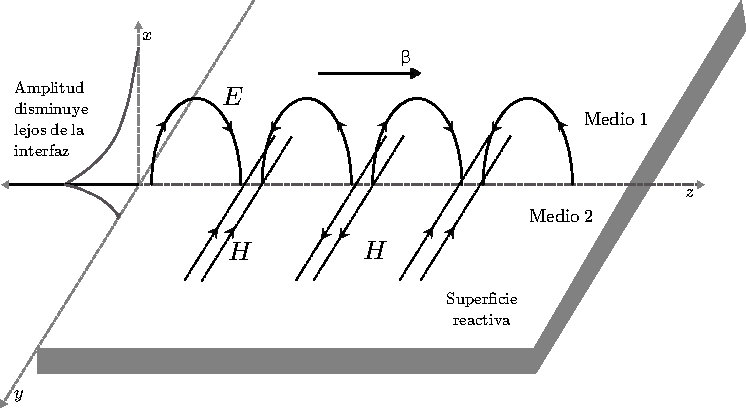
\includegraphics[width=0.8\textwidth]{intro_electro/ondas-superficie-3d.pdf}
	%\input{Figures/intro_electro/onda-superficie-incidencia-brewster3.pdf_tex}
	\caption{Representación gráfica del comportamiento de una onda de superficie TM sobre una interfaz reactiva.}
	\label{fig:onda-superficie-3d}
\end{figure}

Si se considera que una onda plana incide con ángulo de Brewster (concepto desarrollado en el anexo \ref{sec:incidencia-onda-plana-interfaz}) en modo TM sobre una interfaz entre dos medios de bajas pérdidas ($\epsilon'' \ll \epsilon'$), cada uno con una permitividad eléctrica $\epsilon_i$ y una permeabilidad magnética $\mu_i$, $i=1,2$, como indica la figura \ref{fig:onda-superficie-brewster}, no existirá energía reflejada. De esta forma, toda la energía incidente es entregada a la interfaz, y se obtienen las expresiones \ref{eq:ondas-superficie-campos}, donde no existen componentes reflejadas y donde T es el factor de transmisión. Con el fin de simplificar dichas ecuaciones, se considera que el medio 1 es aire, de modo que $\epsilon_1 = \epsilon_0$, $\mu_1 = \mu_0$ y, en consecuencia, $\eta_1 = \eta_0$.

\begin{figure}[htp]
	\centering
	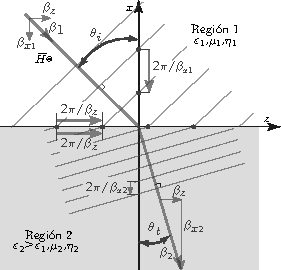
\includegraphics[width=0.7\textwidth]{intro_electro/onda-superficie-incidencia-brewster.pdf}
	%\input{Figures/intro_electro/onda-superficie-incidencia-brewster3.pdf_tex}
	\caption{Ilustración del comportamiento de una onda plana durante la incidencia TM con ángulo de Brewster. Las rectas paralelas representan los frentes de onda, es decir, son rectas de fase constante. Es importante destacar que la longitud de onda paralela a la interfaz, $2\pi/\beta_z$, se mantiene constante a ambos lados, dado que sobre la interfaz se intersecan las rectas de fase constante.}
	\label{fig:onda-superficie-brewster}
\end{figure}

\begin{subequations}
	\label{eq:ondas-superficie-campos}
	\begin{align}
	{H_1}_y &= A e^{-j\ (z\; \overbrace{\gamma_1\;\sin \theta_i}^{\gamma_z} - x\; \overbrace{\gamma_1\;\cos \theta_i}^{\gamma_{x_1}})},\;\; x>0 & j\omega\epsilon E_x &= -\frac{\partial H_y}{\partial z}, \\
	{H_2}_y &= A T e^{-j\; (z\; \overbrace{\gamma_2\; \sin \theta_t}^{\gamma_z} - x\; \overbrace{\gamma_2\; \cos \theta_t}^{\gamma_{x_2}})},\;\; x<0   & j\omega\epsilon E_z &= -\frac{\partial H_y}{\partial x} .
	\end{align}
\end{subequations}

La componente longitudinal de los vectores de onda, $\gamma_z$, es igual a ambos lados de la interfaz, como se muestra en la figura \ref{fig:onda-superficie-brewster} (en términos de $\beta_z$, ya que no se consideran pérdidas), de modo que

\begin{equation}
	\gamma_{1} \; \sin \; \theta_i = \gamma_{z} = \gamma_2 \; \sin \; \theta_t.
\end{equation}

Las componentes normales a la interfaz, que llamaremos $\gamma_{x_i}$, $i=1,2$, mostradas también en la figura \ref{fig:onda-superficie-brewster}, deben cumplir que

\begin{align}
	\label{eq:condicion-componentes-normales-ondas-superficie}
	& \gamma_{x_1}^2 + \gamma_z^2 = \gamma_1^2 &\text{y} &&\gamma_{x_2}^2 + \gamma_z^2 = \gamma_2^2.
\end{align}

Las impedancias de onda en ambas regiones se obtienen como la relación entre los campos tangenciales a la interfaz sobre la que se incide, de modo que

\begin{subequations}
\label{eq:impedancia-onda-superficie}
\begin{align}
	Z_1 = \frac{{E_z}_1}{{H_y}_1} = \eta_0 \; \cos\; \theta_i &\implies Z_1 = \frac{\gamma_{x_1}}{\gamma_1} \eta_0, \label{eq:impedancia-onda-incidente-onda-sup}\\
	Z_2 = \frac{{E_z}_2}{{H_y}_2} = \eta \; \cos \; \theta_t &\implies Z_2 = \frac{\gamma_{x_2}}{\gamma_2} \eta. \label{eq:impedancia-onda-transmitida-onda-sup}
\end{align}
\end{subequations}

Para poder considerar que toda la energía de la onda incidente se transmite desde el primer medio al segundo, debe suceder que las impedancias de onda a ambos lados de la interfaz sean iguales ($Z_1 = Z_2$). Igualando las ecuaciones \ref{eq:impedancia-onda-incidente-onda-sup} y \ref{eq:impedancia-onda-transmitida-onda-sup}, se deduce\footnote{Al igualar las expresiones de las impedancias de onda, se obtiene $\frac{\gamma_{x_1} \eta_0}{\gamma_1} = \frac{\gamma_{x_2} \eta_2}{\gamma_2}$. Recordando que $\gamma_1=\omega \sqrt{\mu_0 \epsilon_0}$, $\gamma_2=\omega \sqrt{\mu_0 (\epsilon'-j\epsilon'')}$, $\eta_0 = \sqrt{\mu_0 / \epsilon_0}$ y $\eta = \sqrt{\mu_0 / (\epsilon'-j\epsilon'')}$, se deduce que la relación entre $\gamma_{x_1}$ y $\gamma_{x_2}$ es compleja: $\gamma_{x_1}\; (\epsilon' - j \epsilon'') = \gamma_{x_2} \epsilon_0$, de modo que en forma general se puede considerar que tanto $\gamma_{x_1}$ como $\gamma_{x_2}$ son complejos.} que, en forma general, si el medio sobre el que se incide tiene pérdidas, entonces $\gamma_{x_1}$ y $\gamma_{x_2}$ son complejos. De esta manera, $\gamma_{x_1} = \beta_{x_1} - j\alpha_{x_1}$ y $\gamma_{x_2} = \beta_{x_2} - j\alpha_{x_2}$, lo que significa que además de avanzar en fase, la onda pierde energía, pues tiene un comportamiento evanescente, de modo que el vector de Poynting tiene una componente en la dirección perpendicular a la interfaz, que se atribuye al consumo de energía de la misma \cite{Barlow:SurfaceWaves}. Dado que $\vec{\gamma_1} = \vec{\gamma_{z_1}} + \vec{\gamma_{x_1}}$, resulta conveniente considerar que la constante de propagación, $\gamma_{z_1} = \beta_{z_1} - j \alpha_{z_1}$, posee también un valor complejo.

El campo magnético queda, entonces, expresado como:

\begin{equation}
	H_y =
	\left\lbrace
	\begin{aligned}
		A e^{-j\beta_z z -\alpha_{z_1} z + j\beta_{x_1}x - \alpha_{x_1}x}, \quad x>0, \\
		A e^{-j\beta_z z -\alpha_{z_2} z + j\beta_{x_1}x + \alpha_{x_2}x}, \quad x<0. \\
	\end{aligned}
	\right.
\end{equation}

Se observa que los planos de fase constante, en el aire, son los correspondientes a las exponenciales imaginarias de la ecuación anterior, $\beta_z z - \beta_{x_1}x = cte$, y se muestran en la figura \ref{fig:onda-superficie-brewster}. Los planos de amplitud constante se obtienen considerando las exponenciales decrecientes de las expresiones, de forma que $\alpha_{z_1}z + \alpha_{x_1}x = cte$, que para el caso analizado en la figura \ref{fig:onda-superficie-brewster}, son rectas con pendiente negativa (no mostradas en la figura). Esto es así porque en la expresión se considera que existen pérdidas en la dirección $z$ paralela a la interfaz. De no haber pérdidas, los planos de amplitud constante resultan paralelos a la misma.

Para bajas pérdidas, $\alpha_{z_i}$, $i=1,2$, será pequeño, por lo que habrá baja atenuación para la onda que se desplaza en dirección $z$, pero debido a que $\alpha_{x_1}$ y/o $\alpha_{x_2}$ también serán bajas, la energía no estará concentrada cerca de la interfaz.



Si se considera una superficie con una impedancia de onda para polarización TM normalizada respecto de $\eta_0$, $Z_s = R_s + j X_s$, independiente del ángulo de incidencia, entonces, al igualar la impedancia de onda a la impedancia de superficie, y teniendo en cuenta las igualdades de la ecuación \ref{eq:impedancia-onda-superficie}, resulta, en el caso TM,

\begin{align}
	\gamma_{x_1} & = \gamma_1 \frac{Z_1}{\eta_0} = \gamma_1 Z_s = \gamma_1 R_s + j \gamma_1 X_s, \label{eq:h1-onda-superficie}\\
	\gamma_z &= \beta_z - j\alpha_z =\sqrt{(\gamma_1^2 - \gamma_{x_1}^2)} = \gamma_1 \sqrt{1+X_s^2 - R_s^2 - 2jR_s X_s}. \label{eq:beta-onda-superficie}
\end{align}

La gráfica de las componentes real e imaginaria de $\gamma_z$ se muestra en la figura \ref{fig:beta-reactancia-TM}. Se puede observar que, cuando la reactancia es inductiva (valores positivos de $X_s$), $\alpha_z$ presenta valores positivos, por lo que habrá atenuación en la dirección de propagación $z$ ([a] en la figura) \footnote{Esto se debe a que si el campo eléctrico en la dirección $y$ se escribe como se indica en la ecuación \ref{eq:ondas-superficie-campos}, $\gamma_z=\beta_z-j\alpha_{z_i}, i=1,2$ y $\gamma_{x_1} = \beta{x_1}+j\alpha_{x_1}$, el exponente se expresa como $-j(\beta_z-j\alpha_{z_1})z + j(\beta_{x_1}+j\alpha_{x_1})x$. Para dirección de propagación $z$, con $z>0$, la componente de atenuación del exponente de la expresión dada resulta en $-\alpha_{z_i} z, i=1,2$. Para que el comportamiento resulte decreciente, $\alpha_{z_i}$ debe ser mayor a $0$.}. Esto significa que, a mayor reactancia, habrá una mayor disminución de la amplitud del campo a medida que la onda se desplace por la interfaz (aumenta el valor de $z$). Sin embargo, la mayor variación en el coeficiente de atenuación se observa con el cambio de valor de la resistencia, $R_s$ ([b] en la figura).

Si la reactancia es nula, un valor de $\beta_z$ se obtiene sólo si la resistencia es muy baja o nula ([c] en la figura). Esto significa que sobre una superficie puramente resistiva, sólo habrá propagación de ondas de superficie cuando la resistencia sea inferior a un umbral dependiende de los medios materiales ($\beta_z=0$, [d] en la figura). Cuando ese umbral de resistencia es superado, el valor de la constante de propagación paralela a la interfaz se anula.

El comportamiento de $\gamma_{x_1}$ (la componente ortogonal a la superficie), descripto en la ecuación \ref{eq:h1-onda-superficie} también regula el comportamiento de la onda de superficie, dado que si la magnitud de la parte imaginaria de $\gamma_{x_1}$, $\alpha_{x_1}$, es muy pequeña, la onda no estará lo suficientemente cerca de la interfaz para ser guiada por ella. Un valor alto de $\alpha_{x_1}$ se da cuando la reactancia, $X_s$ es inductiva ($X_s>0$), lo cual coincide con el requisito para $\alpha_{z_i}, i=1,2$. Dicho de otra forma, la reactancia de superficie es la responsable del decrecimiento exponencial de la onda al aumentar la distancia con la interfaz que funciona como guía.

Analizando la ecuación \ref{eq:beta-onda-superficie}, se deduce que un producto $R_s X_s$ pequeño dará lugar a atenuaciones pequeñas en la onda de superficie, de modo que para que se propague una onda sobre la interfaz, si se establece $X_s$ grande para obtener un valor de $\beta_z$ grande, se deben disminuir el comportamiento resistivo tanto como sea posible ([e] en la figura).

\begin{figure}[htp]
	\centering
	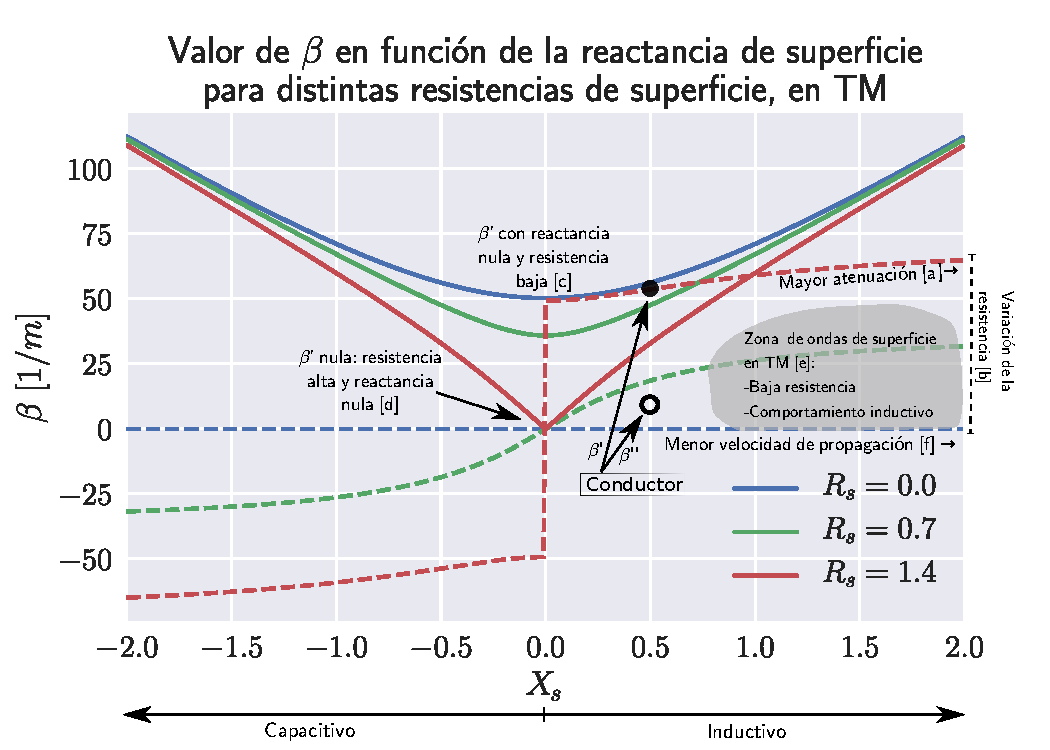
\includegraphics[width=\textwidth]{intro_electro/plot-beta-reactancia-TM.pdf}
	%\input{Figures/intro_electro/onda-superficie-incidencia-brewster3.pdf_tex}
	\caption{Comportamiento de la constante de propagación superficial $\gamma_z$ en función de la resistencia y reactancia superficial para el caso de incidencia TM. Las líneas punteadas representan la parte imaginaria de $\gamma_z$, y las líneas completas representan la parte real, de forma que $\gamma_z = \beta_z - j\alpha_z$.}
	\label{fig:beta-reactancia-TM}
\end{figure}

La velocidad de propagación se obtiene directamente de la componente real de $\gamma_z$ que, si $R_s$ es pequeño y $X_s$ es grande, resulta, a partir de la expresión \ref{eq:beta-onda-superficie}, $\beta_z \approx \beta_1 \sqrt{1+X_s^2}$, de forma que la velocidad de fase es

\begin{align}
	v_p = \frac{\omega}{\beta_z} = \frac{c}{\sqrt{1+X_s^2}}.
\end{align}

En los casos en que la componente reactiva de la impedancia de superficie es grande, el valor de la velocidad de propagación es menor al de la luz (denotado como [f] en la figura).

%%%%%%%%%%%%%%%%%

Cuando la interfaz es de tipo aire-conductor, la componente inductiva de la impedancia de superficie (relacionada a la profundidad de penetración) resulta igual a la componente resistiva, de forma que \cite{Fernandez:Electromag}

\begin{align}
	\eta &= \frac{1+j}{\sigma \delta}.
\end{align}
 
Aplicando las ecuaciones \ref{eq:beta-onda-superficie}, se obtiene que\footnote{Considerando que $\gamma=\omega\sqrt{\epsilon \mu}$, $\eta_0=\sqrt{\epsilon_0}/\sqrt{\mu_0}$ y que $\delta=\sqrt{\frac{2}{\omega \mu_0 \sigma}}$, se observa que $\gamma/\eta_0=\frac{\omega \sqrt{\epsilon_0 \mu_0}}{\frac{\sqrt{\epsilon_0}}{\mu_0}}=\omega \mu_0$, por lo que se puede expresar a $\delta$ como $\frac{2 \eta_0}{\gamma \sigma}$.}

\begin{align}
	\gamma_x &= \gamma_1 (1+j) \sqrt{\frac{\gamma_1}{2 \sigma Z_0}}, \\
	\gamma_z &= \gamma_1 \sqrt{1-\frac{j \gamma_1}{\sigma Z_0}} \approx \gamma_1 - \frac{j  \gamma_1^2}{2 \sigma Z_0}.
\end{align}

En general, un plano conductor soporta ondas de superficie, y la atenuación en la dirección de propagación es muy baja (ver figura \ref{fig:beta-reactancia-TM}), pero no es capaz de lograr una atenuación en la dirección normal al mismo tal que la energía se mantenga concentrada en la superficie para poder ser utilizada como guía de ondas, debido a que la conductividad es muy alta (lo que disminuye el valor de ${\alpha_x}_1$). Para lograr que la energía de la onda decaiga rápidamente lejos de la interfaz es necesario aumentar notoriamente la reactancia de la superficie, para lo que se suele agregar al conductor una capa dieléctrica, que además no aumenta considerablemente la resistividad.

Para el caso de ondas de superficie en modo TE, los campos están dados por la ecuación \ref{eq:campo-electrico-superficie-TE}. La impedancia de onda, en tanto, queda expresada como indica la ecuación \ref{eq:impedancia-onda-superficie-TE}. Considerando que, para evitar reflexiones, la impedancia de superficie tiene que ser igual a la impedancia de onda, se obtiene la expresión para la constante de propagación en el sentido perpendicular a la interfaz mostrada en la ecuación \ref{eq:h1-onda-superficie-TE}, donde nuevamente la impedancia de superficie del conductor es $Z_s = R_s +jX_s$.

\begin{equation}
	\label{eq:campo-electrico-superficie-TE}
	\begin{aligned}
		E_y = A e^{j\gamma_x x-j\gamma_z z}, \qquad j\omega \mu_0 H_z = -\frac{\partial E_y}{\partial x}, \qquad j\omega \mu_0 H_x = \frac{\partial E_y}{\partial z}.
	\end{aligned}
\end{equation}

\begin{align}
	\label{eq:impedancia-onda-superficie-TE}
	Z_1 = \frac{E_y}{H_z} = -\frac{\omega \mu_0}{\gamma_{x_1}} = -\frac{\eta \gamma_1}{\gamma_{x_1}}.
\end{align}

\begin{align}
	\label{eq:h1-onda-superficie-TE}
	\gamma_{x_1} = -\frac{\gamma_1}{Z_s} = -\gamma_1 \frac{R_s}{{R_s^2 + X_s^2}}-j\frac{X_s}{R_s^2 + X_s^2}.
\end{align}

Se observa que para que el valor de $\alpha_{x_1}$ resulte positivo, de manera que se de un decrecimiento exponencial desde la superficie, el valor de $X_s$ tiene que ser negativo, por lo que el comportamiento de la superficie tiene que ser capacitivo.

La segunda condición para la existencia de ondas de superficie, la propagación de los campos, está asegurada si $\gamma_z$ es positivo, y si la atenuación en la dirección de propagación, parametrizada por $\alpha_z$, es baja. La expresión de $\gamma_z$ para el caso TE resulta, a partir de \ref{eq:h1-onda-superficie-TE},

\begin{align}
	\gamma_z = \beta_z-j\alpha_z= \sqrt{(\gamma_1^2 - \gamma_{x_1}^2)} = \frac{\gamma_1}{R_s^2+X_s^2} \sqrt{1+X_s^2 - R_s^2 + 2jR_s X_s}. \label{eq:beta-onda-superficie-TE}
\end{align}

Gráficas de la expresión anterior se muestran en la figura \ref{fig:beta-reactancia-TE}, donde se pueden observar valores de $\beta_z$ y $\alpha_{z_1}$ en función de la reactancia $X_s$, para algunos valores de resistencia de superficie $R_s$. Resulta importante destacar que para valores en que $X_s$ es negativa (reactancia capacitiva), el valor de $\alpha_z$ es físicamente realizable, ya que da lugar a un decrecimiento exponencial, y no a un incremento. Por otro lado, al contrario que en el caso de las ondas TM, a medida que la reactancia capacitiva aumenta en módulo, la constante de propagación tiende a estabilizarse en lugar de crecer linealmente, aunque sí decrece la constante de atenuación $\alpha_z$. Cuando la resistencia de superficie es muy baja, los valores de $\beta_z$ para reactancia $X_s$ nula tienden a ser muy altos. Cuando los valores de resistencia aumentan ligeramente, al igual que en el caso TM, el valor de $\beta_z$ se vuelve nulo, lo que obliga a presentar un comportamiento capacitivo para la propagación de ondas de superficie en modo TE.


\begin{figure}[htp]
	\centering
	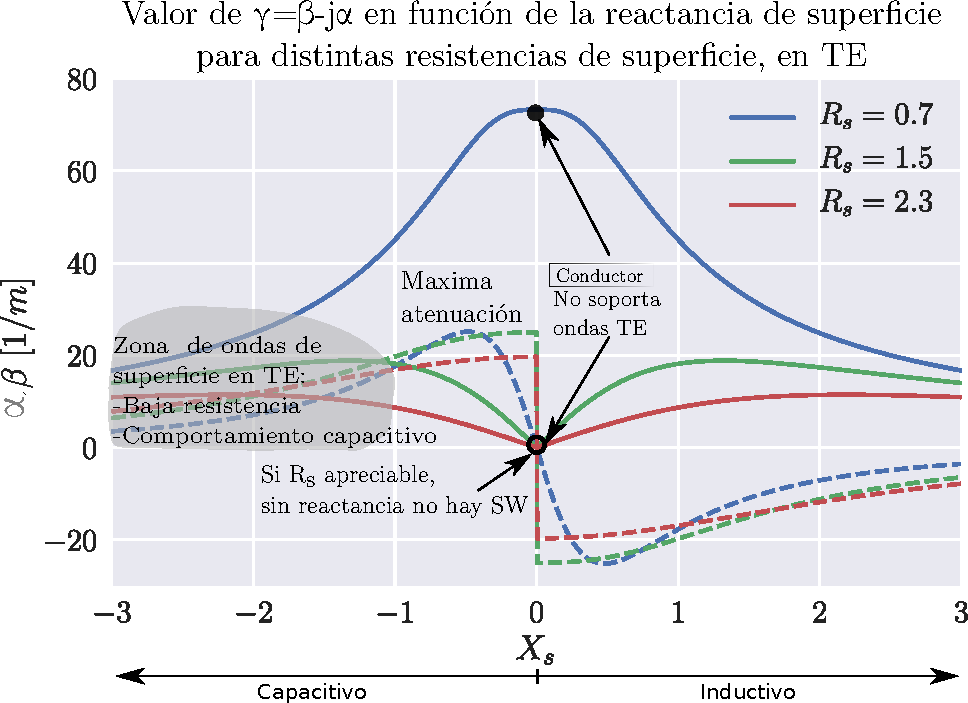
\includegraphics[width=\textwidth]{intro_electro/plot-beta-reactancia-TE.pdf}
	%\input{Figures/intro_electro/onda-superficie-incidencia-brewster3.pdf_tex}
	\caption{Comportamiento de la constante de propagación superficial $\gamma_z$ en función de la resistencia y reactancia superficial para el caso de incidencia TE. Las líneas punteadas representan la parte imaginaria de $\gamma_z$, y las líneas completas representan la parte real, de forma que $\gamma_z = \beta_z - j\alpha_z$.}
	\label{fig:beta-reactancia-TE}
\end{figure}

Entre las distintas formas de lograr que una interfaz conductor-aire permita el guiado de ondas de superficie, una de las más efectivas consiste en el recubrimiento de la superficie metálica por una capa dieléctrica fina, como se muestra en la figura \ref{fig:thin-dielectric-coating}.

\begin{figure}[htp]
	\centering
	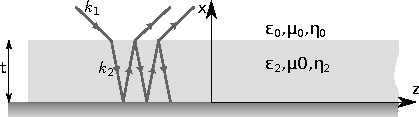
\includegraphics[width=0.7\textwidth]{intro_electro/incidencia-coated-conductor.pdf}
	\caption{Incidencia sobre un conductor recubierto por un dieléctrico.}
	\label{fig:thin-dielectric-coating}
\end{figure}

Para el caso TM, si se considera que el campo magnético tiene la forma de la ecuación \ref{eq:campo-magnetico-TM} en el espacio libre circundante a la estructura, entonces el campo magnético en el interior del dieléctrico resultará de la forma expresada en la ecuación \ref{eq:campo-magnetico-interior-diel-TM}, donde se cumple que $\gamma_{x_1}^2 + \gamma_z^2 = \gamma_1^2$ y $\gamma_{x_2}^2 + \gamma_z^2 = \gamma_2^2 = \epsilon_r \gamma_1^2$.

\begin{align}
	\label{eq:campo-magnetico-TM}
	H_{1_y} = A e^{j\gamma_{x_1} x - j \gamma_z z},\quad x>h.
\end{align}

\begin{align}
	\label{eq:campo-magnetico-interior-diel-TM}
	H_{2_y} = [B e^{j\gamma_{x_2} x} + C e^{-j\gamma_{x_2} x}] e^{-j\gamma_z z},\quad  0\leq x \leq h.
\end{align}

Dado que en toda interfaz las componentes tangenciales de los campos se conservan, y a que las componentes tangenciales del campo eléctrico sobre el conductor se anulan, se deduce que $H_{2_y}$ es un coseno, y se obtienen\footnote{De la ecuación \ref{eq:campo-magnetico-TM} se deriva el campo eléctrico, utilizando la ecuación de Ampère. Al establecer la condición que indica que sobre la interfaz con el conductor no existe campo eléctrico paralelo a la superficie del mismo (se asume un conductor perfecto), se concluye que el valor de B y de C en la ecuación \ref{eq:campo-magnetico-interior-diel-TM} coinciden. Aplicando la condición de continuidad de las componentes tangenciales de los campos sobre la interfaz aire-dieléctrico, se obtiene una relación entre los valores de A y B. Queda expresado el siguiente sistema de ecuaciones:
\begin{equation*}
	\begin{bmatrix}
		-j \gamma_{x_1} e^{-j \gamma_{x_1} h} & -2 \gamma_{x_2}/\epsilon_{r_2} \sin(\gamma_{x_2} h) &  \\
		 -e^{-j \gamma_{x_1} h} & 2 \cos (\gamma_{x_2} h)
	\end{bmatrix}
	\begin{bmatrix}
		A \\
		B
	\end{bmatrix}
	=
	\begin{bmatrix}
		0 \\
		0
	\end{bmatrix}
\end{equation*}

Para que la solución no sea trivial, el determinante de la matriz del sistema tiene que ser nula, lo que da como resultado $\gamma_{x_2} \tan (\gamma_{x_2} h) = -j \gamma_{x_1} \epsilon_{r_2}$.
} las expresiones \ref{eq:solucion-ondas-sup-tm-tan} y \ref{eq:solucion-ondas-sup-tm-h}.


\begin{align}
	\label{eq:solucion-ondas-sup-tm-tan}
	\gamma_{x_2} \tan (\gamma_{x_2} h) = -j \gamma_{x_1} \epsilon_{r_2}, \\
	\gamma_1^2 (\epsilon_{r_2}-1) = \gamma_{x_2}^2 - \gamma_{x_1}^2.
	\label{eq:solucion-ondas-sup-tm-h}
\end{align}

Considerando que $\gamma_{x_1}$ es puramente imaginario positivo\footnote{Un análisis general requiere considerar $\gamma_{x_1}$, $\gamma_{x_2}$ y $\epsilon_2$ como complejos, de manera que se puedan tener en cuenta las pérdidas. Para simplificar el desarrollo, se puede asumir que, dado que se trata de ondas de superficie, la parte imaginaria de $\gamma_{x_1}$ deberá ser negativa, de manera que a mayor distancia de la interfaz, la intensidad de los campos decrezca exponencialmente. La parte real de $\gamma_{x_1}$, si bien puede existir, a efectos del estudio del comportamiento de la onda de superficie en la dirección de propagación, puede obviarse. Por otro lado, si se considera que el ancho del dieléctrico, $h$, es muy pequeño, de forma que se pueda considerar que $\tan(\gamma_{x_2} h) \approx \gamma_{x_2} h$, entonces la expresión \ref{eq:solucion-ondas-sup-tm-tan} resulta aproximadamente $\gamma_{x_2}^2 h = -j \gamma_{x_1} \epsilon_{r_2}$. Asumiendo, por lo explicado antes, que $\gamma_{x_1}$ es valor puramente imaginario positivo, el valor de $\gamma_{x_2}$, obtenido de $\gamma_{x_2}^2 h = \gamma_{x_1} \epsilon_{r_2}$, deberá ser real. Al argumento no descarta la existencia de valores complejos de $\gamma_{x_1}$ y $\gamma_{x_2}$, sino que permite una validación intuitiva del desarrollo posterior.}, la ecuación \ref{eq:solucion-ondas-sup-tm-h} se puede expresar como $\gamma_1^2 (\epsilon_{r_2}-1) = \gamma_{x_2}^2 + |\alpha_{x_1}|^2$. Si se multiplica esta nueva expresión por $h^2$ y a la expresión \ref{eq:solucion-ondas-sup-tm-tan} por $h$, se obtienen dos expresiones que dan lugar a un sistema de ecuaciones trascendentales que se pueden resolver gráficamente, dado que representan una esfera de radio $\gamma_1 h \sqrt{\epsilon_{r_2}-1}$ y una tangente:

\begin{equation}
	\label{eq:sistema-ondas-superficiales-TM}
	\begin{cases}
		(\gamma_{x_2} h)^2 + (\alpha_{x_1} h)^2 = (\epsilon_{r_2} - 1) (\gamma_1 h)^2\\
		\gamma_{x_2} h \tan (\gamma_{x_2} h) = |\alpha_{x_1}| \epsilon_{r_2} h.
	\end{cases}
\end{equation}

Para el caso TE, la solución es similar, y en este caso las expresiones resultan (considerando, nuevamente, que $\gamma_{x_1}$ es puramente imaginario positivo, es decir, $\gamma_{x_1} = \alpha_{x_1}$):

\begin{equation}
	\label{eq:sistema-ondas-superficiales-TE}
	\begin{cases}
		(\gamma_{x_2} h)^2 + (\alpha_{x_1} h)^2 = (\epsilon_{r_2} - 1) (\gamma_1 h)^2 \\
		\gamma_{x_2} h \cot (\gamma_{x_2} h) = -|\alpha_{x_1}| \epsilon_{r_2} h.
	\end{cases}
\end{equation}

Las soluciones se pueden obtener gráficamente para ambos casos, mediante la intersección de las curvas correspondientes a las ecuaciones del sistema. Las gráficas, para distintas frecuencias, se muestran en la figura \ref{fig:intersecciones-tm-te}. Se puede observar que, dado que $|\alpha_{x_1}|h$ no puede tomar valores negativos, las intersecciones que se dan en esas condiciones no son válidas como soluciones del sistema planteado, bajo las hipótesis consideradas.

A medida que aumenta la frecuencia, el valor del radio de los círculos aumenta. Se observa que siempre existe, al menos, un modo TM de propagación sobre el plano de tierra, dado que todas las intersecciones entre las curvas ocurren para valores de $|\alpha_{x_1}| h$ mayores a 0, como se muestra en la figura \ref{fig:soluciones-TM-tan-implicita-zoom}. Para frecuencias en que el radio del círculo genera que el mismo intersecte a más secciones de la curva tangente, aparecerían modos de propagación superiores.

Para el caso TE, se observa que para frecuencias bajas no existe solución válida, como se muestra en la figura \ref{fig:soluciones-TE-tan-implicita-zoom}, por lo que no hay un modo fundamental TE por debajo de la frecuencia de corte, que se da para $f_c = c/(4 h  \sqrt{\epsilon_{r_2}}-1)$, que en el caso graficado es de aproximadamente 25 GHz.

Para el caso de FR4, en el rango de frecuencias de interés para este trabajo, no existe, entonces, propagación de ondas de superficie de polarización TE, por lo que el análisis del modo TM reviste mayor importancia.


\begin{figure} [H]
	\centering 
	\subfigure[TM]{
		\label{fig:soluciones-TM-tan-implicita}
		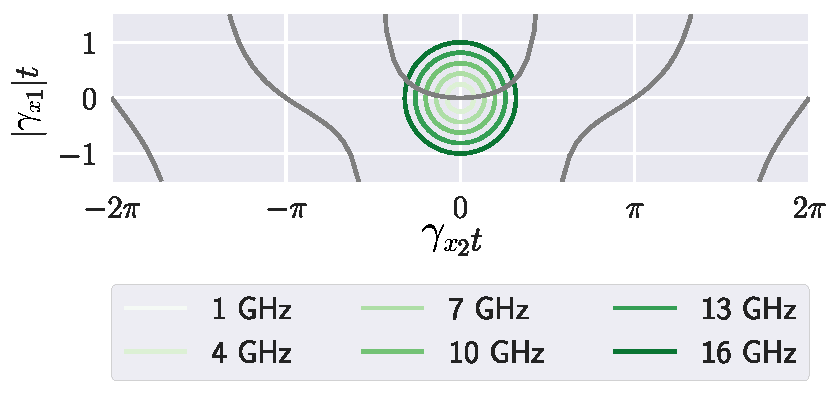
\includegraphics[width=0.48\textwidth]{intro_electro/TM-tan-implicito}}
	\subfigure[TE]{
		\label{fig:soluciones-TE-tan-implicita}
		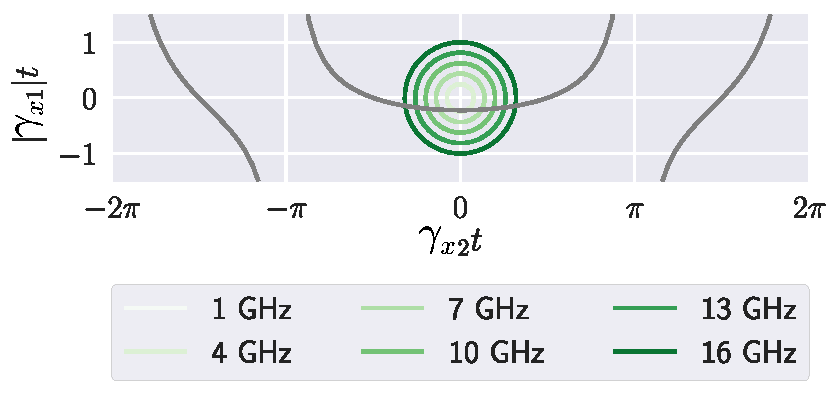
\includegraphics[width=0.48\textwidth]{intro_electro/TE-tan-implicito}}
	\subfigure[Zoom para modo TM]{
		\label{fig:soluciones-TM-tan-implicita-zoom}
		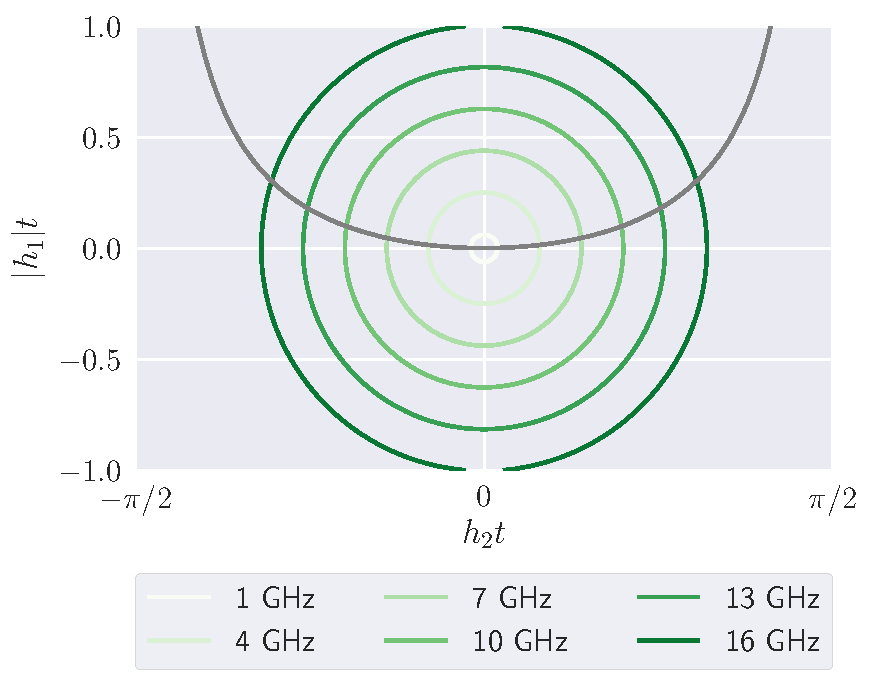
\includegraphics[width=0.48\textwidth]{intro_electro/TM-tan-implicito-zoom}}
	\subfigure[Zoom para modo TE]{
		\label{fig:soluciones-TE-tan-implicita-zoom}
		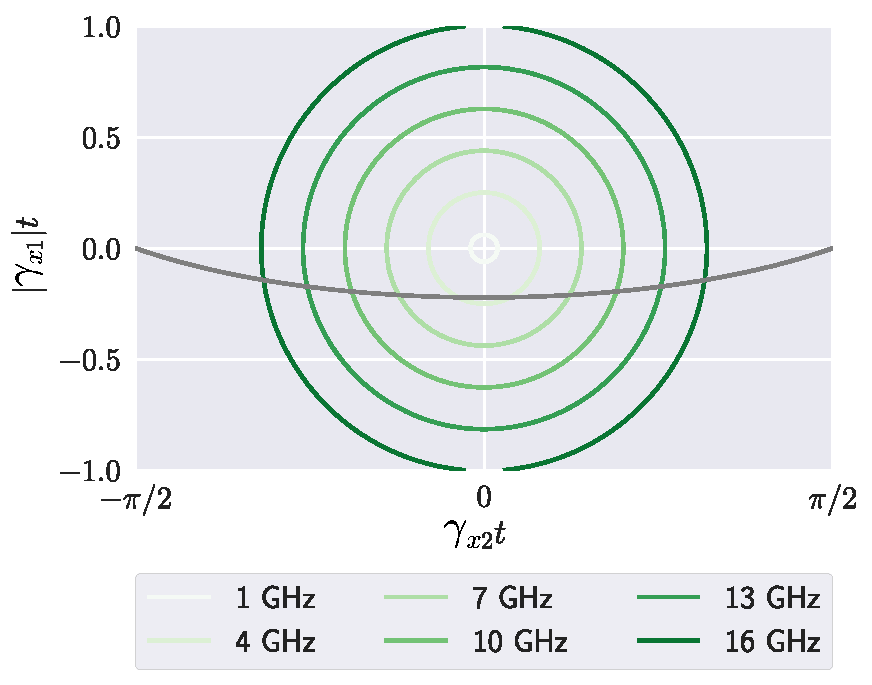
\includegraphics[width=0.48\textwidth]{intro_electro/TE-tan-implicito-zoom}}
	\caption{Curvas de los sistemas de ecuaciones que describen la existencia de ondas superficiales TM y TE, para distintas frecuencias, resuelto para el caso en que el dieléctrico es FR4 ($\epsilon_r = 4.5$).}
	\label{fig:intersecciones-tm-te}
\end{figure}

Obtenidos los valores de $\gamma_{x_1}$ ($\alpha_{x_1}$) y $\gamma_{x_2}$, se obtienen los campos del modo correspondiente de la onda de superficie \cite{Pozar:MwEngineering}. En particular, para el análisis del comportamiento de la impedancia, las expresiones de los campos tangenciales a la interfaz resultan de mayor interés, dado que permiten obtener las impedancias de onda en el aire y el dieléctrico, como se indica en las expresiones \ref{eq:impedancia-no-normalizada-aire} y \ref{eq:impedancia-no-normalizada-FR4}.

\begin{subequations}
	\begin{align}
		H_{y_1} &= A e^{j\gamma_{x_1}(x-h)-j\gamma_{z} z}, &E_{z_1} &= \frac{A \gamma_{x_1}}{\omega \epsilon_0} e^{j\gamma_{x_1}(x-h)-j\gamma_{z} z} &\implies& Z_1 = \frac{\gamma_{x_1}}{\omega \epsilon_0} = j\frac{\alpha_{x_1}}{\omega \epsilon_0}, \label{eq:impedancia-no-normalizada-aire}\\
		H_{y_2} &= 2 B \cos(\gamma_{x_2} x) e^{j\gamma_{z} z}, &E_{z_2} &=  \frac{-2 B \gamma_{x_2} \sin(\gamma_{x_2} x)e^{-j\gamma_{z} z}}{j \omega \epsilon_0 \epsilon_{r_2}} &\implies& Z_2 = \frac{j\gamma_{x_2} \tan(\gamma_{x_2} x)}{\omega \epsilon_0 \epsilon_{r_2}}. \label{eq:impedancia-no-normalizada-FR4}
	\end{align}
\end{subequations}

Normalizando respecto de la impedancia intrínseca del vacío, $\eta_0$, se obtiene, considerando $\theta_t$ el ángulo de transmisión desde el aire al dieléctrico que recubre el plano conductor,

\begin{align}
	\frac{Z_{1}}{\eta_0} &= j\frac{\alpha_{x_1}}{\omega \epsilon_0 \eta_0} = j\frac{\gamma_1 \cos\theta_i}{\omega \epsilon_0 \eta_0} = j\cos \theta_i, \\
	\frac{Z_{2}}{\eta_0} &= j\frac{\gamma_{x_2} \tan \gamma_{x_2} x}{\omega \epsilon_0 \epsilon_{r_2} \eta_0} = j\frac{\gamma_2 \cos\theta_t \tan(\gamma_2 x \cos\theta_t)}{\omega \epsilon_0 \epsilon_{r_2} \eta_0} = j \frac{\cos \theta_t}{\sqrt{\epsilon_{r_2}}}\tan(\gamma_2 x \cos\theta_t).
\end{align}

Una onda incidente desde el aire, para evitar reflexiones y, por lo tanto, radiación desde la superficie que soporta una onda de superficie, debe estar adaptada a la impedancia de superficie que presenta el dieléctrico, que resulta de evaluar $Z_2/\eta_0$ en la superficie, por lo que

\begin{align}
	\label{eq:impedancia-superficie-tm-teorica}
	Z_s^{TM} = j \frac{\cos \theta_t}{\sqrt{\epsilon_{r_2}}}\tan(\gamma_2 h \cos\theta_t).
\end{align}


\begin{figure} [H]
	\centering 
	\subfigure[$Z_s^{TM}$ en función del ancho del dieléctrico, para una permitividad dieléctrica relativa de $4.5$ y en incidencia perpendicular.]{
		\label{fig:zstm-ancho-diel}
		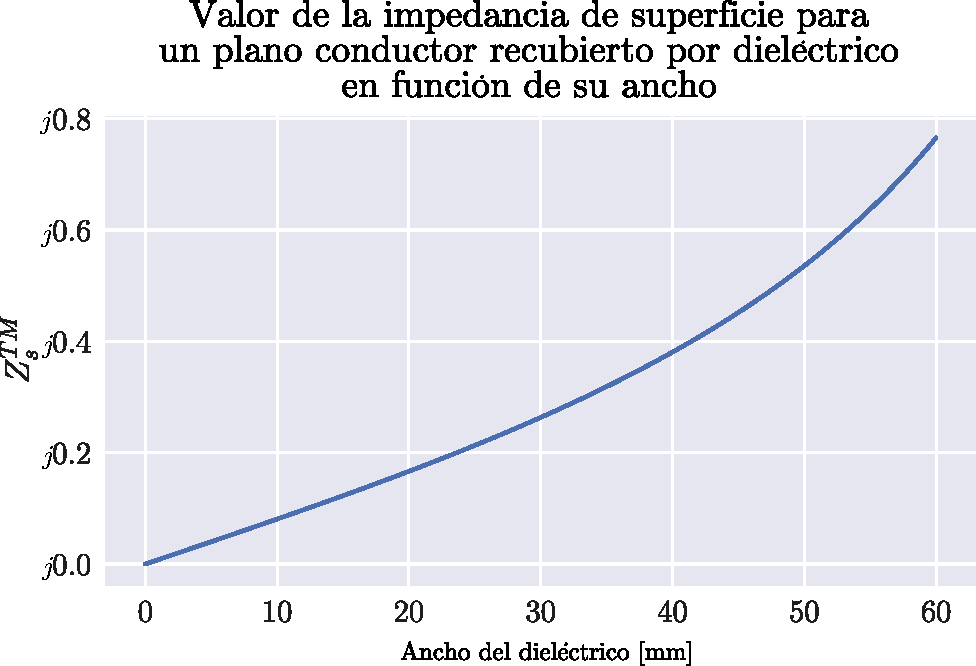
\includegraphics[width=0.45\textwidth]{intro_electro/plot-zstm-funciont.pdf}}
	\hspace{5mm}
	\subfigure[$Z_s^{TM}$ en función de la permitividad dieléctrica, para un ancho de dieléctrico de $1.6\;mm$ y en incidencia perpendicular.]{
		\label{fig:zstm-permit-diel}
		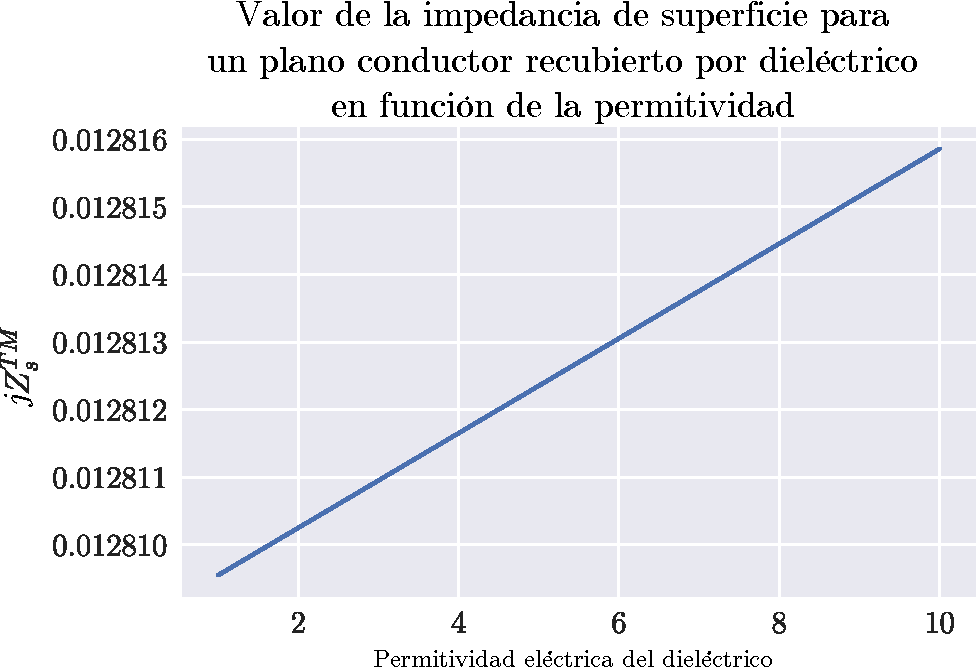
\includegraphics[width=0.45\textwidth]{intro_electro/plot-zstm-funcioner.pdf}}
	\\
	
	\subfigure[$Z_s^{TM}$ en función del ángulo de incidencia, para un ancho de dieléctrico de $1.6\;mm$ y una permitividad de $4.5$.]{
		\label{fig:zstm-angulo-incidencia}
		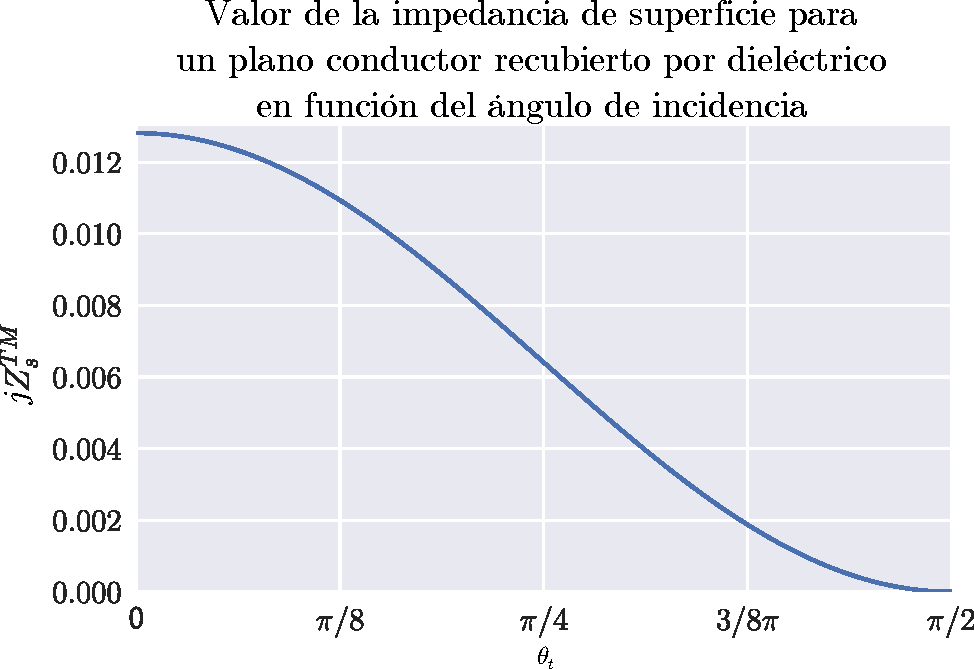
\includegraphics[width=0.45\textwidth]{intro_electro/plot-zstm-funciontheta.pdf}}
	\caption{Valor de la impedancia de superficie en función de sus parámetros.}
	\label{fig:Zstm-parametros}
\end{figure}

%% GRAFICAR!!! \theta_r puede ser obtenida por la ley de snell. Vemos que no es independiente del ángulo de incidencia. Barlow dice que son del mismo orden de magnitud los efectos viejos (prof de penetracion) y los nuevos (coating). Pagina 332. Carita triste.

% Barlow parece contar cosas sobr la velocidad de fase, y más dealnte sobre el lauching y el angulo de brewster complejo. LEER para completar.

Esta impedancia es puramente imaginaria positiva\footnote{Si el dieléctrico presentara pérdidas, existiría también un término real \cite{Barlow:SurfaceWaves}, por lo que, además de facilitar la propagación de ondas de superficie, si el dieléctrico tiene bajas pérdidas, no aumenta la resistencia de superficie. Además, esta componente inductiva se debe sumar al efecto producido por la componente inductiva de la impedancia de superficie del conductor, debida a la existencia de una profundidad de penetración.}, por lo que tiene un comportamiento inductivo, permitiendo la formación de ondas de superficie en modo TM, dado que la constante de atenuación $\alpha_{x_i}, i=1,2$ logra que el campo se concentre cerca de la superficie. Los valores de $\beta_z$ y $\alpha_z$ no se ven modificados, pues el aporte del dieléctrico a la reactancia no es lo suficientemente alto. El ángulo $\theta_t$ se obtiene de las relaciones de Snell (\ref{eq:snell_law_second}), por lo que se deduce que, al contrario que en el caso del conductor sin recubrimiento dieléctrico, el comportamiento es dependiente del ángulo de incidencia, como se muestra en la figura \ref{fig:zstm-angulo-incidencia}. Por otro lado, en la figura \ref{fig:zstm-ancho-diel} se puede observar que el valor de la impedancia crece a medida que aumenta el ancho del dieléctrico, volviéndose más inductiva, de forma similar a la que se da cuando aumenta la permitividad (figura \ref{fig:zstm-permit-diel}).

Para el caso TE, los campos paralelos a la superficie son:

\begin{align}
	E_{y_1} &= A e^{-j\gamma_{x_1}(x-h)-j\gamma_z z}, &H_z &= -\frac{A \gamma_{x_1}}{\omega \mu_0} e^{-j\gamma_{x_1}(x-h)-j\gamma_z z}. \notag \\
	&\implies Z_{1} = -\frac{\gamma_{x_1}}{\omega \mu_0}, \\
	E_{y_2} &= A \sec{(\gamma_{x_2} h)} \cos{(\gamma_{x_2} x)} e^{-j \gamma_z z}, &H_{z_2} &= -\frac{A \gamma_{x_2} e^{j\gamma_z z}}{j\omega \mu_0} \sec{(\gamma_{x_2} h)} \sin(\gamma_{x_2} x), \notag \\
	&\implies Z_{2} = \frac{j\cot(\gamma_{x_2} x)}{\gamma_{x_2} \omega \mu_0}.
\end{align}

Siguiendo la misma metodología que en el caso TM, igualando ambas impedancias, se obtiene

\begin{align}
	Z_s^{TE} = j\frac{\cot(\gamma_2 \cos \theta_t)}{\gamma_2 \cos\theta_t \;\omega \mu_0}.
\end{align}
% Queda explicar qué pasa con el coating -> ubicar también los puntos en el dibujito, para saber por dónde es que nos movimos.


% Engheta, pagina 289
% Rahim (tesis), pagina 28
% Collin, capitulo de Surface waveguides, pag 697
% Paper de Barlow.
% Pozar, pag 138
% Tesis de Kovacs, pagina 8
% Tesis de Zheng, apendice A, pag 48. Interfaces con diel y con metales.


\section{Líneas de transmisión}
\label{sec_lineas_de_transmision}
%%%%

%  Cuando los metamateriales son homogéneos, pueden ser representados por líneas de transmisión unidimensionales, donde la dirección representa cualquier dirección en el material (Caloz, Itoh).

La teoría de líneas de transmisión representa el paso intermedio entre el estudio de campos electromagnéticos y de circuitos de parámetros concentrados, permitiendo considerar el fenómeno de propagación de ondas como una extensión de la teoría de circuitos (aplicable cuando la longitud eléctrica del circuito es mayor a la longitud de onda de operación), o como una solución particular de las ecuaciones de Maxwell \cite{Pozar:MwEngineering}.

Las líneas de transmisión son redes de parámetros distribuidos, donde las corrientes y las tensiones, en contraposición a los circuitos de parámetros concentrados, pueden variar en magnitud y fase, debido a la dimensión física del circuito. El análisis de una línea se puede llevar a cabo estableciendo el comportamiento de los trozos infinitesimales que la componen, dispuestos en cascada para formar la estructura final, de forma que cada uno de ellos se pueda modelar utilizando circuitos de parámetros concentrados independientes de la frecuencia, estableciendo, entonces, impedancias $Z'$ ($\Omega/m$) y admitancias $Y'$ ($S/m$) por unidad de longitud, como se muestra, de forma general, en la figura \ref{fig:TL-equivalente}.

\begin{figure}[htp]
	\centering
	\begin{circuitikz} \draw
		(0,0) -- (1,0)node[midway,scale=2,fill=white]{$\cdots$} -- (7,0)
		(0,2) -- (1,2)node[midway,scale=2,fill=white]{$\cdots$} 
			to [R,l=$R \Delta z$] (3,2)
			to [L,l=$L'_R \Delta_z$] (5,2) 
			to [C,l=$C'_L / \Delta_z$] (7,2)
			to [C,l=$C'_R \Delta_z$] (7,0)
		-- (9,0) to [L,l_=$L'_L / \Delta_z$] (9,2)
		-- (7,2)
		(9,2) -- (11,2)
			to [R,l=$R / \Delta_z$] (11,0)
			-- (9,0)
		(11,0) -- (12,0) -- (13,0)node[midway,scale=2,fill=white]{$\cdots$}
		(11,2) -- (12,2) -- (13,2)node[midway,scale=2,fill=white]{$\cdots$};
	\end{circuitikz}  	
	\caption{Circuito equivalente de porción de línea de transmisión.}
	\label{fig:TL-equivalente}
\end{figure}

La impedancia y la admitancia por unidad de longitud se pueden expresar como indican las expresiones de la ecuación \ref{eq:impedancia-admitancia-TL}. Se debe tener en cuenta que los subíndices R y L se deben al comportamiento de \enquote{mano izquierda}\footnote{La expresión \enquote{material de mano izquierda} fue utilizada por primera vez por físico ruso Viktor Velesago en 1967, cuando propuso la posibilidad de la existencia de materiales en que la propagación de ondas se daría de forma que el campo eléctrico, el campo magnético y el vector de propagación formaran una triada de mano izquierda \cite{Caloz:ElectromagneticMetamaterials}.} o \enquote{mano derecha} asociado a cada componente. Si $L'_R$ y $C'_R$ son nulos, existe sólo un comportamiento \enquote{de mano izquierda}, donde las velocidades de fase y de grupo son antiparalelas, y donde tanto la permitividad eléctrica $\epsilon$ como la permeabilidad magnética $\mu$ son negativas, de forma que el índice de refracción también lo sea, dando lugar a una propagación de ondas en sentido inverso. Cuando $L'_L$ y $C'_L$ son nulos, el comportamiento es denominado \enquote{de mano derecha}, y es el que corresponde a propagación de onda comúnmente analizada. Las componentes que corresponden al comportamiento de mano izquierda son, por sí solas, de existencia física imposibles, dado que las que generan comportamiento de mano derecha aparecen naturalmente por efectos constructivos. Las resistencias del circuito, por otro lado, representan las pérdidas dieléctricas y conductoras.


\begin{align}
\label{eq:impedancia-admitancia-TL}
Z' &= j \left(\omega L'_r - \frac{1}{\omega C'_L} \right), & Y' =j \left(\omega C'_R - \frac{1}{\omega L'_L} \right).
\end{align}

Una descripción completa del análisis del caso general, que describe el comportamiento de numerosos metamateriales, se puede consultar en \cite{Caloz:ElectromagneticMetamaterials}. En adelante se analizará únicamente el caso tradicional, de mano derecha, ya que es el que se aplica al tipo de estructura analizado en este trabajo.

Considerando una línea de transmisión que representa un comportamiento puramente de mano derecha, obteniendo el circuito equivalente de un infinitesimal de línea de la figura \ref{fig:TL-equivalente}, aplicando las leyes de Kirchhoff, dividiendo por $\Delta z$ y aplicando el límite para $\Delta z \rightarrow 0$, para obtener expresiones diferenciales, se obtienen las ecuaciones del telegrafista, expresadas en la ecuación \ref{eq:Telegrafista}, tanto en el dominio del tiempo como de la frecuencia \cite{Fernandez:Electromag}. La solución simultánea de ambas ecuaciones tiene un comportamiento de onda, expresado en \ref{eq:ec-onda-TL}, donde $\gamma$ es la constante de propagación, cuyo valor se expresa en \ref{eq:gamma-tl}.

\begin{align}
	\label{eq:Telegrafista}
	\left. \begin{array}{rr@{\mskip\thickmuskip}l}
	\frac{\partial v(z,t)}{\partial z} & = -R i(z,t) - L \frac{\partial i(z,t)}{\partial t}\\
	\frac{\partial i(z,t)}{\partial z} & = -G v(z,t) - C \frac{\partial v(z,t)}{\partial t}
	\end{array}\right\} \quad \implies \quad \left\{\begin{array}{r@{\mskip\thickmuskip}l}
	\frac{dV(z)}{dz} & = -(R+j\omega L)I(z) \\
	\frac{dI(z)}{dz} & = -(G+j\omega C)V(z).
	\end{array}\right.
\end{align}


\begin{equation}
\begin{aligned}
	\frac{d^2 V(z)}{dz^2} + \gamma^2 V(z) = 0, \\
	\frac{d^2 I(z)}{dz^2} + \gamma^2 I(z) = 0.
\end{aligned}
\label{eq:ec-onda-TL}
\end{equation}

\begin{align}
	\label{eq:gamma-tl}
	\gamma = -j\alpha + \beta = \sqrt{-ZY} = \sqrt{-(R+j\omega L)(G+j\omega C)}.
\end{align}

En base a esta constante de propagación, es posible definir la velocidad de fase $V_p$ como

\begin{align}
	V_p = \frac{\omega}{\beta},
\end{align}

que para el caso sin pérdidas resulta

\begin{align}
	\label{eq:vprop-linea-ideal}
	V_p = \frac{\omega}{\omega \sqrt{LC}} = \frac{1}{\sqrt{LC}}.
\end{align}

Las ecuaciones de onda tienen como solución la superposición de una onda en dirección $+z$ y otra en dirección $-z$, tanto para la tensión como para la corriente, con velocidad de fase $\omega/\beta$. La relación entre las componentes de onda que viajan en dirección positiva se conoce como impedancia característica, $Z_0$, definida, según los parámetros de una línea de transmisión, en la ecuación \ref{eq:TL-impedancia-caracteristica}.
 
\begin{align}
	\label{eq:TL-impedancia-caracteristica}
	Z_0 = \frac{V_0^+}{I_0^+} = \sqrt{\frac{R+j\omega L}{G+j\omega C}}.
\end{align}

Cuando una línea de transmisión es terminada en una impedancia arbitraria $Z_L$, se producen fenómenos de transmisión y reflexión de potencia, de manera análoga al caso de incidencia de campos electromagnéticos sobre interfaces entre medios de impedancias intrínsecas diferentes, analizado en el apéndice \ref{sec:incidencia-onda-plana-interfaz}. Existe, también en este caso, un coeficiente de reflexión $\Gamma$, definido como la relación entre la tensión reflejada y la tensión incidente, como indica la ecuación \ref{eq:coef-reflexion-tl}. Cuando el coeficiente de transmisión es nulo, se dice que la carga está adaptada, de modo que $Z_L = Z_0$.

\begin{align}
	\label{eq:coef-reflexion-tl}
	\Gamma = \frac{V_0^-}{V_0^+} = \frac{Z_L-Z_0}{Z_L+Z_0}.
\end{align}

Si se generaliza el concepto de coeficiente de transmisión a cualquier punto de la línea, y no únicamente al nodo donde se coloca la carga $Z_L$, se obtiene el coeficiente de reflexión para cualquier punto $l$ de la línea a partir del que corresponde al nodo de carga, ubicado en la posición 0, como se indica en la ecuación \ref{eq:coef-reflexion-tl-generalizado}.

\begin{align}
\label{eq:coef-reflexion-tl-generalizado}
\Gamma(l) = \Gamma e^{-2j\gamma l} = \Gamma e^{-2j\beta l} e^{-2\alpha l}.
\end{align}

La impedancia de entrada también varía con la distancia a la carga, de forma que:

\begin{align}
Z_{in} = \frac{V(-l)}{I(-l)} = Z_0 \frac{Z_L +Z_0 \tanh \gamma l}{Z_0 + Z_L \tanh \gamma l}.
\end{align}

En la figura \ref{fig:Zin-Gamma-funcionDistancia-TL} se puede observar una gráfica de $\Gamma$ y $Z_{in}$ en función de la distancia a la carga, para una línea de impedancia característica $Z_0$ de $50 \; \Omega$, con una carga de $100 \; \Omega$, considerando pérdidas y constante de propagación arbitrarias.

\begin{figure}[htp]
	\centering
	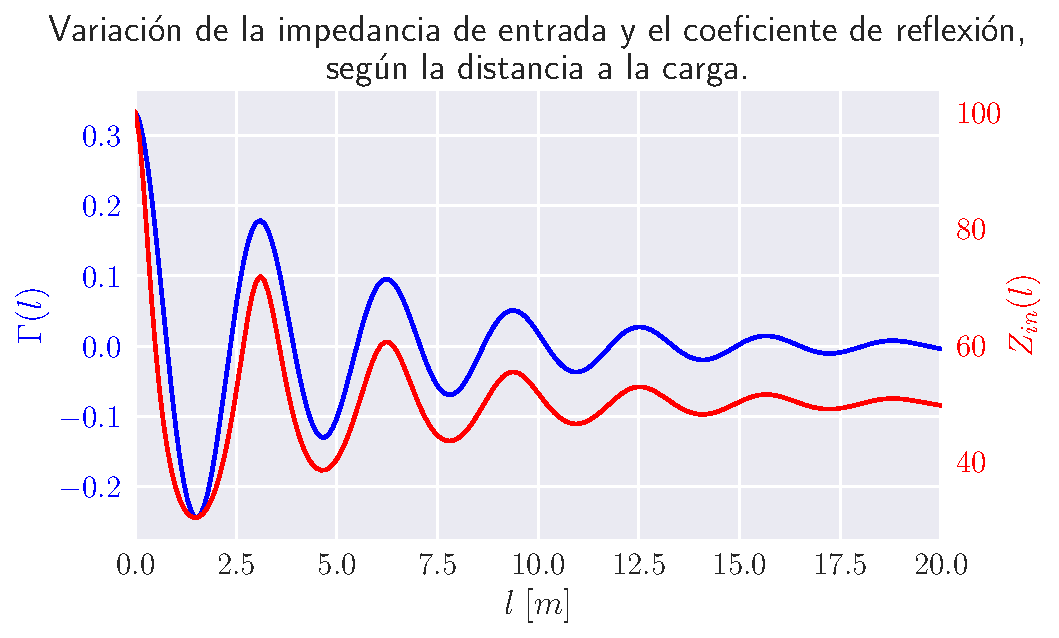
\includegraphics[width=0.8\textwidth]{intro_electro/Zin-Gamma-funcionDistancia-TL.pdf}
	\caption{Impedancia de entrada y coeficiente de reflexión en función de la distancia a la carga, en una línea de transmisión de $50 \Omega$.}
	\label{fig:Zin-Gamma-funcionDistancia-TL}
\end{figure}

En base a este análisis, resulta útil conocer la matriz de transferencia $ABCD$ que corresponde a una línea de transmisión ideal. La misma relaciona las tensiones y corrientes en un nodo con las de otro de forma que

\begin{figure}[htp]
	\centering
	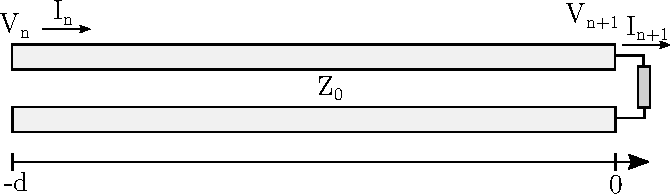
\includegraphics[width=0.8\textwidth]{intro_electro/lineaTransmision-d.pdf}
	\caption{Línea de transmisión con carga.}
	\label{fig:TL-con-carga}
\end{figure}

\begin{align}
\begin{bmatrix}
A & B \\
C & D
\end{bmatrix}
\begin{bmatrix}
i_n \\
v_n
\end{bmatrix}
=
\begin{bmatrix}
i_{n+1} \\
v_{n+1}
\end{bmatrix}.
\end{align}

La deducción de los componentes de la matriz de transferencia requiere del análisis de las ondas incidentes y reflejadas que inciden sobre terminales ubicados a una distancia $d$ de la carga, que puede ser un cortocircuito (para obtener los valores de $B$ y $D$) o un abierto (de donde se pueden deducir los valores de $A$ y $C$).

Dado que la tensión reflejada vista a distancia $d$ de la carga, $V^{-}(d)$, se calcula como $-Z_0 I^{-}$, y que la tensión total sobre dicho nodo resulta de la suma de ambas tensiones (la incidente y la reflejada), para el caso de una carga cortocircuito ($Z_L = 0$), donde la tensión sobre la carga es $V_{n+1} = 0$, resulta que:

\begin{align}
	\Gamma = -1 \implies V(d) = V_n e^{-j\gamma d} - V_n e^{j\gamma d} = 2 j V_n \sin(\gamma d) = B, \\
	I_n (d) = I_n e^{-j\gamma d} + I_n e^{j\gamma d} = 2 I_n \cos(\gamma d) = D.
\end{align}

De forma similar, para el caso de una carga de tipo circuito abierto, $Z_L \rightarrow \infty$, $\Gamma = 1$ y

\begin{align}
V(d) = V_n e^{-j\gamma d} + V_n e^{j\gamma d} = 2 V_n \cos(\gamma d) = A, \\
I_n (d) = I_n e^{-j\gamma d} - I_n e^{j\gamma d} = 2 j I_n \sin(\gamma d) = C.
\end{align}

En forma normalizada, la matriz resulta \cite{Pozar:MwEngineering}

\begin{align}
\label{eq:matriz_transferencia_lineaideal}
\begin{bmatrix}
\cos(\gamma d) & \sin(\gamma d) \\
\sin(\gamma d) & \cos(\gamma d)
\end{bmatrix}.
\end{align}


% Venkateswaran, cap 1.
%%%%
\subsection{Línea \textit{microstrip}}

Algunas de las líneas de transmisión más comunes están basadas en tecnologías de circuitos impresos, entre las que se destacan las \textit{striplines} (donde el dieléctrico circundante al conductor es homogéneo), las líneas \textit{microstrip} (donde el dieléctrico circundante es aire en la mitad superior, y un dieléctrico de mayor permitividad en la mitad inferior), y las guías de ondas coplanares (donde el plano de tierra y la línea de señal comparten la misma cara del sustrato). Algunas de ellas son esquematizadas en la figura \ref{fig:strip-line-technology}. Los costos de fabricación de las mismas suelen ser muy bajos, y ofrecen comodidades para la implantación de componentes discretos, aunque en muchos casos se generan modos indeseados, que pueden ser disminuidos manteniendo el espesor del sustrato en valores despreciables respecto de la longitud de onda, lo que los vuelve frágiles. Además, los sustratos dieléctricos suelen presentar pérdidas que modifican el comportamiento de la señal. Las principales aplicaciones se relacionan con el diseño de filtros microondas, acopladores direccionales, transformadores de impedancia, planos de tierra y redes de distribución de energía de circuitos impresos e integrados \cite{Venkateswaran:Thesis}.


\begin{figure}[htp]
	\centering
	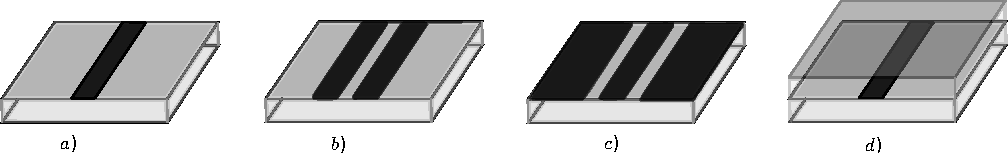
\includegraphics[width=\textwidth]{intro_electro/microstrip-stripline-coplanar.pdf}
	\caption{Tecnologías de líneas de transmisión planares. De izquierda a derecha: \textit{Microstrip}, \textit{twinstrip}, línea coplanar y \textit{stripline}.}
	\label{fig:strip-line-technology}
\end{figure}

Las \textit{striplines}, debido a la homogeneidad del dieléctrico, soportan modos TEM. Las líneas \textit{microstrip}, en cambio, sólo pueden presentar modos TE y TM, aunque en frecuencias bajas tienen un comportamiento que puede denominarse cuasi-TEM, dado que la mayor parte del campo se concentra en el dieléctrico \footnote{Un comportamiento puramente TEM impediría el cumplimiento de la condición de fase en la interfaz, dado que las velocidades de propagación en ambos medios es distinta \cite{Pozar:MwEngineering}}. Un diagrama simplificado de los campos y los parámetros de una línea \textit{microstrip} se muestran en la figura \ref{fig:microstrip-campos}


\begin{figure}[htp]
	\centering
	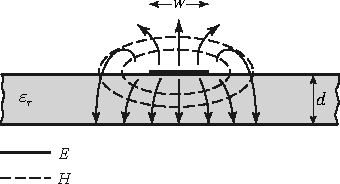
\includegraphics[width=0.5\textwidth]{intro_electro/microstrip-campos.pdf}
	\caption{Campos de una línea \textit{microstrip} [Basado en representación de \cite{Pozar:MwEngineering}].}
	\label{fig:microstrip-campos}
\end{figure}

En general, para simplificar el análisis, se considera que la cinta \textit{microstrip} es una \textit{stripline}, donde el dieléctrico tiene una constante dieléctrica efectiva, menor a la constante dieléctrica del sustrato, pero mayor a la del aire, dependiente del ancho del sustrato, el ancho del conductor y la frecuencia de trabajo. La expresión de esta constante es

\begin{align}
	\epsilon_{eff} = \epsilon_0 \left(\frac{\epsilon_r+1}{2} + \frac{\epsilon_r-1}{2} \left( 1+12 \frac{h}{W} \right)^{-1/2} \right).
	\label{eq:cte-diel-efectiva-microstrip}
\end{align}

\section{Antenas}
\label{subsec_antenas}
%%%%

Una antena es un dispositivo que actúa como fuente de ondas electromagnéticas. Es una interfaz entre el espacio libre y un dispositivo de guiado (como una guía de ondas o una línea de transmisión), y puede ser puede ser modelada como una carga que, en general, está adaptada. Su función es recibir o transmitir energía, usualmente optimizando algunas direcciones, y suprimiendo o disminuyendo su valor en otras, para lo que se utilizan distintas tecnologías, entre las que se destacan las antenas de hilo, de apertura y \textit{microstrip}, muchas veces dispuestas en arreglos y con componentes reflectores \cite{Balanis:Theory}. En este trabajo resultarán de mayor importancia las regiones más cercanas al radiador, y el control del comportamiento de los campos en las mismas modificará el comportamiento en la región de Fraunhoffer.

%%%%
\subsection{Regiones de campo}
\label{subsubsec_regiones_de_campo}
%%%%
El espacio que rodea a una antena se suele dividir en tres regiones: Campo cercano reactivo (donde predominan los campos reactivos), campo de radiación cercano (Fresnel, donde la distribución angular de energía depende de la distancia a la antena) y campo lejano (Fraunhoffer, donde la distribución angular de energía es, en términos prácticos, independiente de la distancia al elemento radiante). En general, se considera que la región de campo lejano se encuentra a distancias mayores a $2D^2/\lambda$, donde D es la máxima dimensión de la antena, y $\lambda$ es la longitud de onda de trabajo.

%%%%
\subsection{Diagramas de radiación}
\label{subsubsec_diag_de_rad}
%%%%
El diagrama de radiación es una representación gráfica o función matemática que representa las propiedades de radiación de una antena como función de las coordenadas espaciales. En general, se especifica para la región de campo lejano, y en función de las coordenadas direccionales $\theta$ y $\phi$, que representan el ángulo de elevación y el azimutal, respectivamente, para una orientación arbitraria del radiador.

En general, se calcula el patrón de potencial o el patrón de campo eléctrico, y se los normaliza respecto de su máximo valor, para luego graficarlos en escala logarítmica o en decibeles.

Sobre el patrón se distinguen lóbulos, clasificados como principal (en la dirección de mayor radiación) y menores (en otras direcciones). El diagrama de radiación de una antena isotrópica, de ser físicamente realizable, se correspondería con una esfera, dado que no existen direcciones privilegiadas. Cuando no existen lóbulos distinguibles en un dado plano, lo cual es común es antenas con simetría cilíndrica, el comportamiento se denomina omnidireccional.
%%%%

\subsection{Impedancia de entrada}
\label{subsec_imp_entrada}
%%%%
La impedancia de entrada de una antena es la que presenta a la línea de transmisión o guía de ondas que la alimenta. En general tiene una componente resistiva y una componente reactiva, de manera que $Z_A = R_A + j X_A$. En general, $R_A$ tiene dos componentes: $R_r$, la resistencia de radiación, y $R_L$, la resistencia de pérdidas. Como en general no coincide con la impedancia característica de la línea de transmisión que la alimenta, se aplican métodos de adaptación de impedancias.
%%%%

\subsection{Arreglos de antenas}
% Ver apunte tesis overleaf

Un arreglo de antenas es un conjunto de antenas dispuestas geométricamente, y alimentadas de manera tal que conformen un único sistema radiante. El primer conjunto de antenas usado extensivamente fue la antena Yagui-Uda, inventada en 1926, cuya fase no puede variarse electrónicamente. Recién durante la Segunda Guerra Mundial se inventaron los conjuntos de antena de fase variable, y a partir de 1950, con la invención de los defasadores de ferrita, la modificación de fase completa fue posible \cite{Stutzman:AntennaTheory}.

El análisis más sencillo del comportamiento de conjuntos de antenas se presenta al analizar uno formado por antenas de iguales propiedades, cuyas amplitudes y fases pueden ser modificados, tanto en transmisión (a través de mecanismos de desfasaje) como en recepción (debido a diferencias e camino y circuitos de desfasaje). En general, el diagrama de radiación se puede calcular en base a la multiplicación del patrón de uno de los elementos y el patrón del arreglo, para el cual se asumen puntos de radiación isotrópicos en la posición de las antenas \cite{Balanis:Theory}.

\begin{figure}[htp]
	\centering
	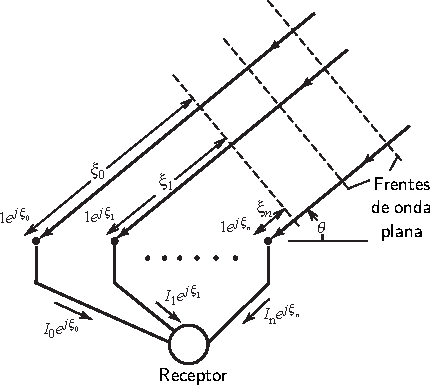
\includegraphics[width=0.5\textwidth]{intro_electro/array-de-antenas.pdf}
	\caption{Incidencia de una onda plana sobre un arreglo de antenas [Basado en la representación del fenómeno en \cite{Balanis:Theory}].}
	\label{fig:rayosincidentes-array}
\end{figure}

El factor de \textit{array}, reemplazando cada elemento por radiadores isotrópicos, se obtiene considerando que una onda plana incide con ángulo $\theta$ sobre el conjunto, como se muestra en la figura \ref{fig:rayosincidentes-array}. Cada elemento es excitado con una fase $\xi_i$, debida a la diferencia de caminos y a las diferencias entre las líneas de transmisión de cada antena, de modo que

\begin{equation}
AF=I_0e^{j\xi_0} + I_1e^{j\xi_1} + ... = \sum_{n=0}^{N-1} I_n e^{j\beta n d cos(\theta)}=\sum_{n=0}^{N-1} I_n e^{jn\Phi}.
\end{equation}

Normalizando y simplificando la expresión, la misma queda

\begin{equation}
	f(\Phi) = \frac{sin(N\Phi/2)}{N sin(\Phi/2)} \qquad (2\pi-\text{periódica}),
\end{equation}

con N la cantidad de elementos radiantes. Se observa que si hay una mayor cantidad de elementos radiantes, los lóbulos, tanto secundarios como primarios, tiende a aumentar. Además, al mismo tiempo, la cantidad de lóbulos secundarios también crece (hay N-1 lóbulos secundarios), al mismo tiempo que disminuye la altura de los mismos \cite{Stutzman:AntennaTheory}.

\subsection{Acoplamiento mutuo}
\label{subsec_acoplamiento}
%%%%
Cuando se considera acoplamiento mutuo entre los elementos del \textit{array}, la multiplicación del patrón de radiación por el patrón del arreglo ya no es válida. Los elementos interaccionan entre sí y alteran sus corrientes, y por lo tanto sus impedancias. La radiación de una antena induce corrientes sobre las antenas cercanas, que también radian e influyen sobre la corriente de la primer antena. Es un efecto de campo cercano.

La impedancia de entrada de un elemento aislado en el espacio se denomina \enquote{Impedancia de elemento aislado}, o simplemente impedancia de antena. La impedancia de entrada de una antena que está dispuesta en un ambiente con elementos activos se denomina \enquote{impedancia activa}, y varía según las excitaciones a las que se someta al arreglo de antena. En general, la caracterización de los elementos radiantes sometidos a efectos de acoplamiento mutuo consisten en la obtención de la \enquote{impedancia pasiva}, que se logra excitando un elemento y conectando a cargas adaptadas los demás.

Hay 3 efectos responsables del acoplamiento mutuo en arreglos de antenas:

\begin{itemize}
	\item Acoplamiento espacial entre elementos.
	\item Acoplamiento espacial por \textit{scattering} en elementos cercanos.
	\item Acoplamiento por la red de alimentación, que puede ser minimizado usando técnicas de acoplamiento apropiadas en cada elemento.
\end{itemize}

Si el acoplamiento en la red de alimentación se minimiza, se puede considerar que cada antena está alimentada independientemente con una tensión $V_m^g$, cuyo generador tiene una impedancia asociada $Z_m^g$. Sobre la antena se genera una diferencia de tensión $V_m$, y una corriente $I_m$, que incluye los efectos de acoplamiento. Un \textit{array} de N elementos es entonces una red de N puertos, representada por la ecuación \ref{eq:Matriz_impedancias_mutuas}, donde todos los elementos que pertenecen a la diagonal de la matriz $Z$ son las impedancias de elemento aislado, mientras que los elementos fuera de la diagonal representan las impedancias mutuas $Z_{mn}$, que no es más que la tensión impresa sobre el elemento $m$ por la corriente $n$, cuando todos los demás terminales están a circuito abierto ($Z_{mn}=V_m/I_n |_{I_i=0\; \forall i \neq n}$, lo que significa que la corriente es nula para todo el cuerpo de la antena). En general estos cálculos se realizan de forma numérica, tras las correspondientes simulaciones, y considerando a las antenas en modo transmisor \cite{Fano:CouplingReceiving}.

\begin{equation} \label{eq:Matriz_impedancias_mutuas}
\begin{bmatrix}
V_1 \\ V_2 \\ \vdots \\ V_N
\end{bmatrix}
=
\underbrace{\begin{bmatrix}
	Z_{11} & Z_{12} & \cdots & Z_{1N} \\
	Z_{12} & Z_{22} & \cdots & Z_{2N} \\
	\vdots & \vdots & \cdots & \vdots \\
	Z_{1N} & Z_{2N} & \cdots & Z_{NN} \\
	\end{bmatrix}}_{Z}
\begin{bmatrix}
I_1 \\ I_2 \\ \vdots \\ I_N
\end{bmatrix}.
\end{equation}

Si suponemos que la antena no excitada tiene una impedancia de carga $Z^g_j$ sobre sus terminales (y que el generador de esa antena está apagado, $V^g_j=0$), la corriente generada sobre el elemento $j$ debido a la radiación del elemento $i$ será tal que $V_j=-Z^g_j I_j$, por lo que

\begin{equation} \label{eq:impmutua}
V_j = -Z^g_j I_j = Z_{jj}I_j + \sum_{i=1, i \neq j}^{N} Z_{ji}I_i.
\end{equation}

En el caso en que se consideren sólo dos antenas, de la ecuación \ref{eq:impmutua} para dos elementos, podemos obtener la expresión de la corriente en el segundo elemento, que da lugar a la expresión de la impedancia total vista por el primer elemento, por efecto propio y de la radiación del segundo, como muestra la ecuación \ref{eq:impedanciamutua}, donde se asumió que la matriz Z es simétrica, y que permite deducir la ecuación \ref{eq:impedanciaAntenaEnArray}, que es la impedancia de entrada de cada elemento, en función de impedancias mensurables.

\begin{equation}
	\label{eq:impedanciamutua}
	\left\{
	\begin{aligned}
		V_1 &= Z_{11} I_1 + Z_{12} I_2 \\
		V_2 = -Z^g_2 I_2 &= Z_{22} I_2 + Z_{21}I_1.
	\end{aligned}
	\right.
\end{equation}

\begin{align}
	\label{eq:impedanciaAntenaEnArray}
	I_2 = \frac{-Z_{21}I_1}{Z_{22}+Z^g_{2}} = \frac{-Z_{12}I_1}{Z_{22}+Z^g_{2}}  \quad \implies \quad
	\frac{V_1}{I_1} = Z_1 = Z_{11} - \frac{(Z_{12})^2}{Z_{22}+Z^g_2}.
\end{align}

%Paper de fano y el cordobeés.
%%%%
%\subsection{Dieléctricos y pérdidas dieléctricas}
%\label{subsec_dielectricos}
%%%%%%%%%%%%%%%%%%%%%%%%%%%%%%%%%%%%
%%%%%%%%%%%%%%%%%%%%%%%%%%%%%%%%%%%%
%%%%%%%%%%%%%%%%%%%%%%%%%%%%%%%%%%%%
%%%%%%%%%%%%%%%%%%%%%%%%%%%%%%%%%%%%
%%%%%%%%%%%%%%%%%%%%%%%%%%%%%%%%%%%%
%\lipsum[2]
% LibroSinNombre, pagina 816
%%%%%%%%%%%%%%%%%%%%%%%%%%%%%%%%%%%%

\subsection{Antenas \textit{microstrip}}
\label{subsec_antenas_microstrip}
%%%%
Las antenas \textit{microstrip} cumplen varias de las especificaciones más importantes que imponen las diversas aplicaciones de antenas: Pueden ser pequeñas, tienen bajo peso, son económicas y fáciles de fabricar, y tienen bajo perfil, lo que permite adaptarlas a numerosos diseños. Suelen, sin embargo, tener un alto Q, ya que funcionan debido a sus propiedades resonantes, suelen tener baja eficiencia, son de baja potencia, y presentan polarización impura.

En general, el diseño de una antena \textit{microstrip} se realiza de forma tal que el máximo de radiación se concentre en la dirección normal al parche (\textit{broadside}), aunque también es posible lograr radiación en dirección paralela al mismo (\textit{end-fire}), dependiendo de la geometría elegida. El sustrato elegido para la fabricación suele influir en el ancho de banda y la eficiencia: Una mayor permitividad dieléctrica genera una menor eficiencia, un menor ancho de banda y un menor acoplamiento con elementos cercanos, debido a que los campos se encuentran contenidos en el sustrato.

Existen múltiples formas de alimentación de una antena \textit{microstrip}, entre las que se destacan la línea microstrip de alimentación, que suele dar lugar a radiación espuria y a polarización cruzada, debido a la asimetría que impone; y la conexión directa de cable coaxil, donde el conductor central del mismo se conecta en un punto del parche, y la malla se conecta al plano de tierra que funciona como reflector, ubicado en la cara opuesta del sustrato.

Existen varios métodos de análisis de antenas \textit{microstrip}, entre los que se destacan, por su sencillez, el modelo de líneas de transmisión y el modelo de cavidades resonantes, principalmente aplicables a parches rectangulares, que son los de interés en este trabajo. Sin embargo, estos métodos no consideran acoplamiento mutuo ni ondas de superficie, por lo que resultan incompletos \cite{Pozar:InputImpedanceMutualCoupling}.
%%%%
\subsubsection{Modelo de líneas de transmisión}
\label{subsubsec_microstrip_modeloLineas}
%%%%
El modelo de líneas de transmisión es el más sencillo y el que ofrece una mayor intuición física, ya que usa los conceptos fundamentales de líneas \textit{microstrip}. Consiste en considerar a la antena como dos aperturas radiantes de ancho $W$ y altura $h$ separadas una distancia $L$ por una línea de transmisión de impedancia característica conocida $Z_0$, cada una de las cuales puede ser representada, en el modelo, como una conductancia $G$ y una susceptancia $B$, como se indica en la figura \ref{fig:circuito-equivalente-antena-ms}, donde la admitancia y la susceptancia se obtienen del modelo de apertura radiante, que puede consultarse en \cite{Balanis:Theory}.

\begin{figure}[htp]
	\centering
	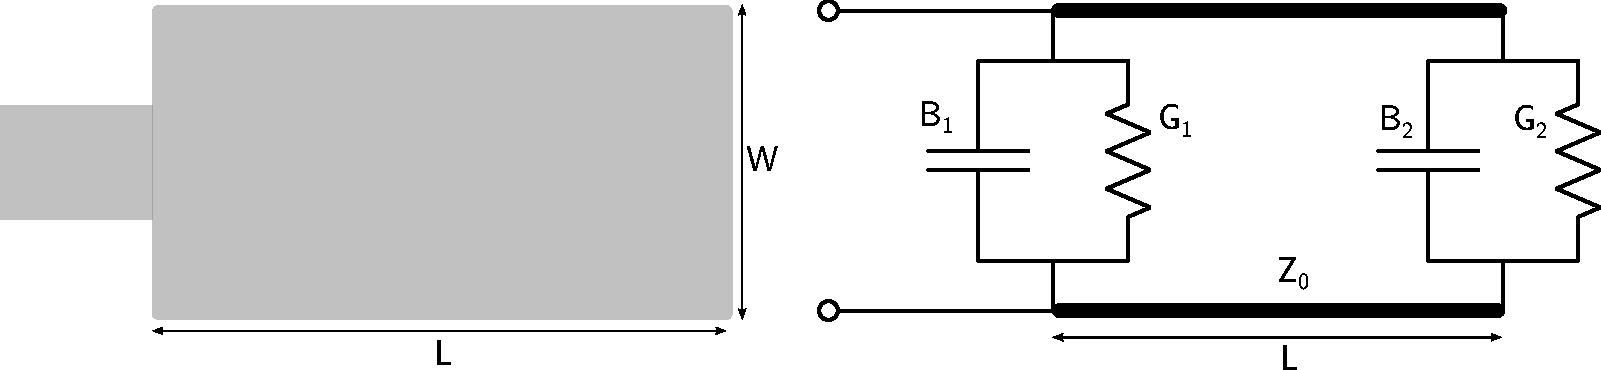
\includegraphics[width=0.8\textwidth]{intro_electro/circuito-equivalente-antena-ms.pdf}
	\caption{Circuito equivalente, según el modelo de líneas de transmisión, de una antena \textit{microstrip}.}
	\label{fig:circuito-equivalente-antena-ms}
\end{figure}



Al igual que en el caso de las líneas \textit{microstrip}, se debe considerar una constante dieléctrica efectivo $\epsilon_{r_{eff}}$, que depende no sólo del ancho del sustrato, sino también de la frecuencia, debido a que a mayor frecuencia hay una mayor concentración de campo sobre el dieléctrico, otorgando mayor prevalencia a la constante dieléctrica del sustrato que a la del aire circundante en el cálculo de la constante efectiva. La expresión es la misma utilizada para líneas \textit{microstrip} (ecuación \ref{eq:cte-diel-efectiva-microstrip}), siempre y cuando $W>h$.

El efecto de \textit{fringing} en los bordes del parche, que da lugar a un aumento del tamaño eléctrico, se modelan mediante la consideración de una extensión en la línea de transmisión que une a las aperturas radiantes, en función de la altura del sustrato. El cambio en la extensión de la línea de transmisión sugiere un cambio en la frecuencia de resonancia de la antena, al mismo tiempo que un mayor ancho de banda, sin una modificación del tamaño físico. En la ecuación \ref{eq:deltaL-antena-microstrip} se muestra una expresión aproximada de la variación del tamaño eléctrico, de forma que la longitud efectiva de la línea de transmisión resulta $L_{eff} = L + 2 \Delta L$. Esta expresión se utiliza para la obtención de la frecuencia de resonancia, como indica la expresión \ref{eq:frec-resonancia-modelo-linea-microstrip} para el modo dominante, $TM_{010}$.

\begin{align}
	\Delta L = h\; 0.412 \frac{(\epsilon_{eff}+0.3)(W/h + 0.264)}{(\epsilon_{eff}-0.258)(W/h +0.8)}.
	\label{eq:deltaL-antena-microstrip}
\end{align}

\begin{align}
	f_{{r}_{010}} = \frac{v_p}{\lambda} = \frac{c/\sqrt{\epsilon_{r_{eff}}}{2*L_{eff}}} = \frac{1}{2 L_{eff} \sqrt{\epsilon_{eff}} \sqrt{\mu_0 \epsilon_0}} = \frac{1}{2 (L+2 \Delta L) \sqrt{\epsilon_{eff}} \sqrt{\mu_0 \epsilon_0}}.
	\label{eq:frec-resonancia-modelo-linea-microstrip}
\end{align}

La impedancia de entrada de una antena \textit{microstrip} depende fuertemente de la posición de la alimentación, además de los valores de $G$ y $B$ de los \textit{slots} radiantes \cite{Balanis:Advanced}. Cuando la alimentación se realiza mediante una cinta \textit{microstrip}, se suele terminar la misma en el interior del parche, a una distancia $y_0$ del borde, como se indica en la figura \ref{fig:antema-microstrip-inset}, permitiendo una mejor adaptación, aunque introduciendo una capacidad de juntura que afecta a la frecuencia de resonancia. La distancia del punto de alimentación al borde del parche será menor a la mitad de la longitud total del parche, en lo que se identificó como \enquote{zona de adaptación} en la misma figura.

\begin{figure} [H]
	\centering
	\subfigure[]{
		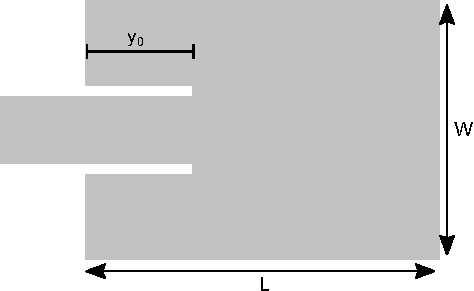
\includegraphics[width=0.48\textwidth]{intro_electro/antena-inset-drawing.pdf}}
	\subfigure[]{
		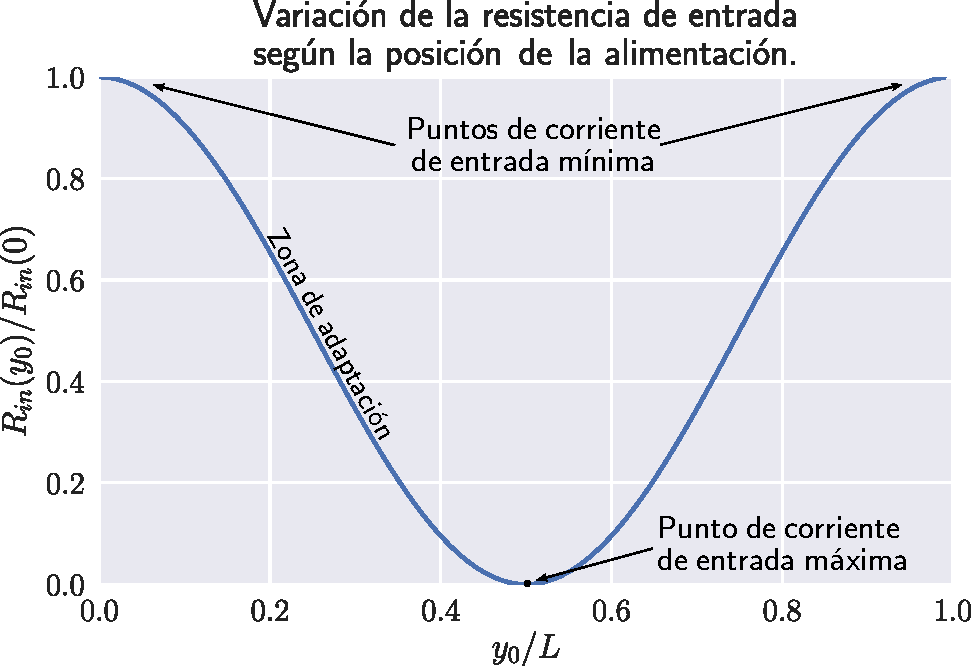
\includegraphics[width=0.48\textwidth]{intro_electro/plot-RinInset.pdf}}
	\caption{Esquema y gráfica del comportamiento de la impedancia de entrada según la posición de la alimentación.}
	\label{fig:antema-microstrip-inset}
\end{figure}


El factor de antena, el ancho de banda y la eficiencia son valores interdependientes, y entre ellos se presenta una relación de compromiso. El factor de antena representa las pérdidas de la misma, en general dominadas por la radiación (relacionada a la conductancia asociada a las aperturas radiantes), la conducción (en función de la conductividad del metal), las pérdidas dieléctricas (expresada según la tangente de pérdidas) y las ondas de superficie (despreciables si el sustrato es demasiado fino). Además, se debe tener en cuenta la adaptación de la antena, que limita fuertemente el ancho de banda de uso. En general, se observa que \cite{Balanis:Theory} a mayor volumen de la antena, el ancho de banda aumenta. Un aumento de la permitividad dieléctrica genera una disminución del ancho de banda, debida a la disminución de los campos de borde (\textit{fringing}) y una disminución de la eficiencia de radiación, dado que da lugar a antenas de menor tamaño. Un sustrato de mayor constante dieléctrica, entonces, da lugar a antenas de menor volumen, lo cual genera un menor ancho de banda.

% LibroSinNombre, pahgina 534
%%%%
\subsubsection{Modelo de cavidades multimodo}
\label{subsubsec_microstrip_modeloCavidades}
%%%%

El modelo de cavidad resonante se utiliza principalmente para predecir el comportamiento en modos superiores de la antena. Para ello se considera que la región dieléctrica bajo el parche consiste en una cavidad cargada dieléctricamente, limitada por conductores eléctricos en las caras superior e inferior, y por conductores magnéticos en las caras laterales. Esta configuración conlleva a una impedancia de entrada puramente reactiva, incompatible con el comportamiento radiante del sistema, pero consistente con el comportamiento de otros parámetros. Para considerar las pérdidas por radiación, se añaden efectos de pérdidas dentro de la cavidad, relacionados con el factor de antena correspondiente.

La consideración de paredes laterales como conductores magnéticos deviene de la consideración de la disposición de las cargas sobre el parche conductor y sobre el plano de tierra, donde se asume que el espesor del dieléctrico es lo suficientemente pequeño como para que no se presenten modos superiores sobre el eje vertical. Las cargas sobre la cara inferior del parche son atraídas por las cargas opuestas correspondientes en el plano de tierra, y su concentración genera una repulsión, hacia la cara superior, a otras cargas de la misma polarización, generando una corriente superficial en cada cara, como se indica en la figura \ref{fig:corrientes-microstrip}. Al disminuir el ancho del sustrato, el efecto de atracción del plano del tierra supera, en magnitud, al efecto de repulsión por la concentración de cargas en la cara inferior del parche, por lo que el flujo decrece, pudiendo considerarse nulo. Dado que el flujo de cargas, a través de los bordes, entre la cara superior y la inferior del parche metálico dispuesto sobre el sustrato, es el responsable del campo magnético tangencial a los bordes, la desaparición de dicho flujo disminuiría considerablemente este campo, permitiendo asumir que las paredes se comportan como conductores magnéticos. La baja altura del sustrato, además, permite considerar sólo las configuraciones TM para las frecuencias de interés, dado que, como se explicó antes, $h<<\lambda$.

\begin{figure}[htp]
	\centering
	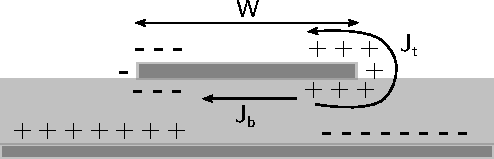
\includegraphics[width=0.4\textwidth]{intro_electro/corrientes-microstrip.pdf}
	\caption{Corrientes sobre el parche en una antena \textit{microstrip}, según el modelo de cavidad.}
	\label{fig:corrientes-microstrip}
\end{figure}

La obtención de los campos se detalla en \cite{Balanis:Advanced}, donde, considerando las hipótesis descriptas antes, asumiendo que el vector de potencial $\vec{A}$ tiene que cumplir la ecuación de Helmholtz (\ref{eq:Helmholtz}), y utilizando separación de variables, se obtienen soluciones para distintos modos, todos transversales magnéticos, con frecuencias de resonancia dadas por \ref{eq:frecRes-modosSup-microstripAntenna}, donde $n$, $m$ y $p$ son los índices del modo. El modo dominante, dado que $h < L$ y $h < W$, es el $TM_{010}$, cuya distribución de campos se muestra en la figura \ref{fig:distribucion-campos-microstrip}.
 
\begin{align}
	(f_r)_{nmp} = \frac{1}{2 \pi \sqrt{\mu \epsilon}} \sqrt{\left(\frac{m\pi}{h}\right)^2 + \left(\frac{n\pi}{L}\right)^2 + \left(\frac{p\pi}{W}\right)^2}.
	\label{eq:frecRes-modosSup-microstripAntenna}
\end{align}

\begin{figure}[htp]
	\centering
	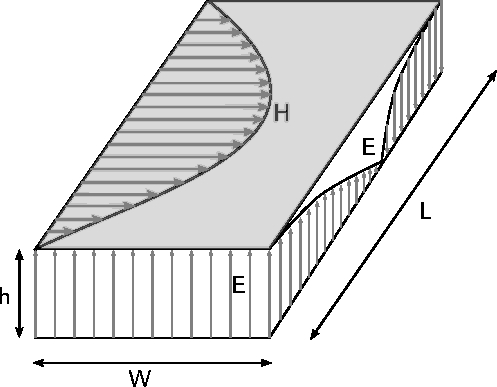
\includegraphics[width=0.4\textwidth]{intro_electro/distribucion-campos-microstrip.pdf}
	\caption{Distribución de campos eléctrico y magnético en la cavidad de \textit{microstrip}, para el modo $TM_{010}$.}
	\label{fig:distribucion-campos-microstrip}
\end{figure}

A pesar de que hay 4 aperturas en una antena \textit{microstrip} rectangular, sólo 2, las radiantes, aportan significativamente a la radiación, dado que lo radiado por las otras dos se cancelan sobre los planos principales. Las paredes separadas aproximadamente $\lambda/2$ tienen campos en direcciones opuestas en el mismo momento, por lo que se suman en la dirección normal al parche, dando lugar a un comportamiento \textit{broadside}.

Un aspecto importante del análisis por el modelo de cavidad radica en las densidades de corriente equivalentes. Según lo descripto antes, existe una corriente, $\vec{J}$, sobre la superficie del parche. Debido a que la polarización es TM, sobre las aperturas radiantes laterales debe existir también una densidad de corriente eléctrica, $\vec{J}_s$, y una densidad de corriente magnética, $\vec{M}_s$, de modo que, en función de los campos en las aperturas,

\begin{align}
	\vec{J}_s &= \hat{n} \times \vec{H}_a, & \vec{M}_s = - \hat{n} \times \vec{E}_a
\end{align}

Según las hipótesis dadas antes, y como se muestra en la figura \ref{fig:distribucion-campos-microstrip}, la magnitud del campo magnético tangencial a las paredes es despreciable, de modo que la corriente sobre las paredes, $\vec{J}_s$, también lo es. La corriente sobre el parche, debido a la baja distancia con el plano de tierra, es baja, por lo que también puede considerarse despreciable. De esta forma, la única densidad de corriente apreciable es $\vec{M}_s$. El efecto del plano de tierra se puede tener en cuenta considerando teoría de imágenes. Según la misma, dado que se trata de un conductor eléctrico, las corrientes magnéticas imagen tienen el mismo sentido que las originales, de modo que la densidad de corriente magnética equivalente resulta el doble que la original, como se expresa en la ecuación \ref{eq:densidad-de-corriente-caras-laterales-microstrip}, y se observa en la figura \ref{fig:densidad-corriente-microstrip}.

\begin{align}
	\label{eq:densidad-de-corriente-caras-laterales-microstrip}
	\vec{M}_s = -2 \hat{n} \times \vec{E}_a.
\end{align}

\begin{figure}[htp]
	\centering
	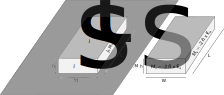
\includegraphics[width=0.8\textwidth]{intro_electro/distribucion-corrientes-microstrip}
	\caption{Densidades de corrientes eléctricas y magnéticas en una antena \textit{microstrip}.}
	\label{fig:densidad-corriente-microstrip}
\end{figure}

Se puede considerar, entonces, que cada apertura actúa como un dipolo magnético con densidad de corriente $\vec{M}_s$. Cuando las aperturas están separadas una distancia de $\lambda/2$, forman un arreglo de dos elementos, que tiene un comportamiento \textit{broadside}.

% Pozar, resonadores, capitulo 6
%%%%

\subsection{Acoplamiento mutuo en antenas \textit{microstrip}}
\label{subsec_acoplamiento_microstrip}
%%%%
El acoplamiento mutuo está determinado principalmente por los campos que existen sobre la interfaz dieléctrico-aire: la onda espacial (decrece como $1/\rho$), los campos cercanos de superior (decreciendo como $1/\rho^2$), la onda de superficie (con dependencia de tipo $1/\rho^{1/2}$) y las ondas de tipo \textit{leaky} (con dependencia del tipo $e^{-Q}/e^{1/2}$) \cite{Balanis:Advanced}. A mayor distancia del elemento radiante fuente, las ondas de superficie son las que tienen carácter dominante, siempre que en esa dirección existan \cite{Alexopoulos:PrintedDipoles}. En general, si la distancia entre los elementos radiantes es grande (mayor a $0.8 \lambda$), la influencia de las ondas de superficie es baja y el acoplamiento es por tanto bajo. Aún así, si el conjunto es grande, la suma de los efectos de los distintos parches puede dar lugar a efectos de acoplamiento significativos, incluso entre elementos no adyacentes \cite{Dodov:SurfaceWavesImpact}. Como en todo conjunto de antenas, el acoplamiento mutuo es función, además de la distancia, de la posición entre los elementos radiantes.

En un \textit{array} planar de antenas se deben considerar la amplitud y la fase de la onda incidente. Si se ubican en forma colineal sobre el plano anche, el acoplamiento mutuo entre las antenas es menor al que se observa si se ubican de forma colineal sobre el plano E (figura \ref{fig:acomplamientoEyH}, \cite{VanLil:TLModelCoupling}, \cite{Pozar:InputImpedanceMutualCoupling}), y el aumento de la distancia entre los parches reduce el acoplamiento \cite{Dodov:SurfaceWavesImpact}. Si los elementos se ubican en forma colineal sobre el plano E, el decrecimiento del parámetro $S_{12}$ es mucho más lento, debido a la presencia de ondas de superficie, comenzando a partir del modo TM, que no posee frecuencia de corte inferior, y aumentando con la aparición de modos TE y TM de orden superior, fruto del aumento de espesor del sustrato y el crecimiento de la constante dieléctrica \cite{Alexopoulos:PrintedDipoles}. La ubicación sobre el plano H genera que las ondas responsables del acoplamiento sean de polarización TE, mientras que la ubicación sobre el plano E genera que las mismas sean de polarización TM, que es la polarización dominante en las antenas \textit{microstrip}. Un aumento en el ancho del sustrato permitiría la aparición de modos TE, generando un mayor acoplamiento en el arreglo sobre el plano H.

\begin{figure}[htp]
	\centering
	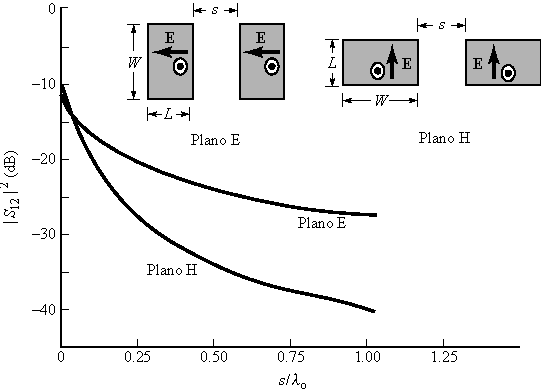
\includegraphics[width=0.8\textwidth]{intro_electro/pozar-acoplamiento.pdf}
	\caption{Acoplamiento mutuo entre antenas \textit{microstrip}, para posición colineal en plano E y plano H. Parámetros: W: 10.57 cm, L: 6.55 cm, h: 0.1588 cm, $\epsilon_r$: 2.55, $f_r$: 1.410 MHz. Fuente: D. M. Pozar, \enquote{Input impedance and mutual coupling of rectangular microstrip antennas}, IEEE Trans. Antennas Propagat. Vol AP-30, No. 6. Noviembre, 1982.}
	\label{fig:acomplamientoEyH}
\end{figure}

Según \cite{Dodov:SurfaceWavesImpact}, los efectos de onda de superficie son importantes cuando el valor de $\epsilon_r$ del sustrato es alto, y si las pérdidas son bajas, la onda de superficie se mantiene en un valor estable cuando se aumenta la distancia \cite{Gonzalo:PerformancePBG}. Esto hace que el acoplamiento mutuo entre las antenas sea mayor, porque existe una onda de superficie notoria. Por otro lado, según \cite{Penard:MutualCouplingMicrostrip}, si el ancho del dieléctrico es bajo, las ondas de superficie son despreciables. Para separaciones pequeñas, los efectos de campo cercano son los que dominan; en la zona intermedia ($0.4\lambda  < d <  0.8 \lambda$), los efectos de la onda espacial directa son visibles, y en la zona más lejana sólo son reconocibles los efectos originados por las ondas de superficie \cite{Alexopoulos:PrintedDipoles}.

La búsqueda de antenas de menor tamaño (aumentando la constante dieléctrica del sustrato) y mayor ancho de banda (aumentando el ancho del dieléctrico) tiene como obstáculo la relación de compromiso con el acoplamiento causado por ondas de superficie, que son amplificadas cuando la constante dieléctrica aumenta o el sustrato es de mayor altura. En el caso de los llamados \textit{phased arrays} de antenas \textit{microstrip}, el acoplamiento mutuo genera, además de modificaciones en el diagrama de radiación, una limitación en el ángulo de escaneo y puntos ciegos \cite{Iluz:PhasedArray}.

%%%%
% LibroSinNombre, pagina 562 y 631


